\chapter{Controlled Characterization of the Liquid State Machine}
\label{chap:lsm}

\section{Introduction and Purpose}
\label{sec:ch3_intro}

This chapter asks how a fixed LIF reservoir responds to controlled synthetic pulses as its membrane decay, firing threshold, temporal window, and readout are varied. The goal is engineering characterization, not a claim that these simplified inputs reproduce EEG or establish performance on clinical data.

Reservoir-computing theory gives conditions under which a sufficiently rich system can approximate time-invariant causal operators with fading memory \cite{Maass2002RealTime,boyd_chua_1985}. These are existence results, not guarantees for the finite reservoir or stimuli used here. The practical task is therefore to document how controllable parameters---membrane decay, firing threshold, network size, and feature extraction---change the observed driven response.

The separation property motivates checking whether different inputs lead to distinguishable reservoir states \cite{Maass2002RealTime}. It does not follow from a single classification result, and a negative finite-time trajectory-divergence estimate does not by itself prove the Echo State Property or separation. The later dynamical analysis reports such estimates descriptively; this chapter makes the narrower measurements shown in its figures and limits its conclusions to the tested synthetic inputs.

The measurements provide provisional settings for the embedding pipeline in Chapter~\ref{chap:embeddings}. Whether those settings transfer to the Stress, Health, and the Psychophysiology of Emotion (SHAPE) EEG summaries is evaluated separately in Chapter~\ref{chap:arspi_net}; the present chapter does not establish that transfer.

Synthetic constant-amplitude pulses are used as controlled probes, not as surrogates for EEG. They make parameter-dependent response patterns easy to inspect, but the design does not identify every causal mechanism and does not include the noise, nonstationarity, or between-person variability of the later data. All quantitative claims in this chapter are limited to these simplified inputs.

The chapter is organized as four experimental modules, each building on the findings of its predecessor. Each module answers a specific question about how hidden temporal order becomes observable, or fails to become observable, under different reservoir operating conditions:
\begin{enumerate}
    \item \textbf{Module 1} (Section~\ref{sec:module1}): \emph{What temporal scale of hidden order does the reservoir preserve?} The membrane decay parameter $\beta$ controls the reservoir's temporal integration window. This module identifies the regime in which the reservoir's fading memory is matched to the timescale of the input's discriminative structure.
    \item \textbf{Module 2} (Section~\ref{sec:module2}): \emph{How does lowering the threshold change the response?} The module contrasts five high-threshold realizations with one low-threshold realization and therefore characterizes response shape, but cannot compare cross-initialization stability between regimes.
    \item \textbf{Module 3} (Section~\ref{sec:module3}): \emph{Which tested temporal windows distinguish the two responses using mean-rate features?} The comparison is limited to two deterministic class responses.
    \item \textbf{Module 4} (Section~\ref{sec:module4}): \emph{Are the two observed synthetic response vectors separable by a linear readout?} The result is a deterministic sanity check, not an estimate of out-of-sample performance.
\end{enumerate}

The reservoir architecture and neuron model are described in Chapter~\ref{chap:background}, Sections~\ref{sec:neuron_models}--\ref{sec:discrete_lif}. Most archived figures in Modules~1--2 use 512 units, fixed random input weights $\mathbf{W}^{\text{in}} \in \mathbb{R}^{512 \times 33}$, and fixed random recurrent weights $\mathbf{W}^{\text{rec}} \in \mathbb{R}^{512 \times 512}$. The original figure-generation script was not retained, and the negative retained potentials in the low-threshold plots show that those figures do not reproduce the audited update, which floors the post-threshold retained membrane at zero. Modules~1--2 are therefore retained as legacy qualitative observations rather than verification of the current implementation. The corrected synthetic classification in Chapter~\ref{chap:embeddings} uses the included NumPy implementation: it emits a spike when the pre-reset membrane reaches threshold, subtracts the threshold, floors the retained membrane at zero, and clears the retained contribution on the next step for units that spiked.

\textbf{Reservoir size.} The figures in this chapter use 512 neurons. Chapter~\ref{chap:embeddings} separately examines a 256-neuron configuration. Results are not assumed to transfer unchanged across sizes; the later configuration is treated as a distinct empirical choice.


%% ===================================================================
%% MODULE 1
%% ===================================================================
\section{Module 1: Impact of the Membrane Time Constant on Reservoir Dynamics}
\label{sec:module1}

\subsection{Theoretical Motivation}

The membrane time constant $\tau_m$ is one important control on how an LIF unit integrates temporal input. It can be viewed in the time domain as a decay constant and, for the subthreshold single-unit approximation, in the frequency domain as a low-pass-filter parameter.

In the subthreshold single-unit approximation, the impulse response is exponential, $h(t)=(1/\tau_m)e^{-t/\tau_m}$ for $t\geq0$. Related time-causal scale-space constructions use cascades of truncated-exponential kernels under specified axioms \cite{lindeberg_2016}; that result should not be read as a uniqueness theorem for the complete recurrent, thresholded reservoir used here. Larger $\tau_m$ gives a wider integration window, while smaller $\tau_m$ gives faster decay.

The corresponding continuous-time linear filter has transfer function $H(f)=1/(1+j2\pi f\tau_m)$ and cutoff $f_c=1/(2\pi\tau_m)$. This description is useful locally, but thresholding, reset, recurrence, and discrete sampling mean that the full reservoir is not simply a bank of identical linear filters.

Information-processing-capacity analyses show that finite reservoirs allocate limited capacity across memory and nonlinear transformations \cite{dambre_2012}. The present sweep does not estimate those capacities, however, so $\beta$ is interpreted only through the observed response persistence rather than as a measured position on a universal memory--nonlinearity curve.

For eventual EEG processing, the discrete reservoir timescale must be considered together with the input sampling and preprocessing. This module does not map simulation steps directly to physiological frequency bands; it sweeps $\beta$ and records response persistence in simulation steps.

\subsection{Experimental Design}

The primary observable is the summed membrane potential across all reservoir neurons:
\begin{equation}
    V_{\text{summed}}[t] = \sum_{i=1}^{N_{\text{res}}} M_i[t]
    \label{eq:v_summed}
\end{equation}
which serves as a convenient aggregate state variable for comparing reservoir operating regimes. It is not claimed to be physiologically equivalent to a local field potential.

A standardized input pulse of amplitude 0.8 was applied to the first 5 of 33 input features, starting at time step 20 and lasting 10 steps, within a total simulation of 150 time steps. The $\beta$ parameter was varied across four values: $\beta \in \{0.01, 0.02, 0.05, 0.10\}$, corresponding to approximate time constants $\tau_m \approx \{100, 50, 20, 10\}$ simulation steps (see Section~\ref{sec:discrete_lif} for the exact $\beta$--$\tau_m$ relationship). For each condition, both $V_{\text{summed}}[t]$ traces and individual-neuron membrane potential heatmaps were recorded for qualitative and quantitative comparison.

\subsection{Results}

The variation of $\beta$ changed response persistence in the plotted realization (Figure~\ref{fig:summed_beta_response}). At $\beta=0.01$ the summed membrane potential remained elevated through the 150-step simulation; progressively larger $\beta$ values produced faster return toward baseline. This is finite-epoch persistence, not evidence of long-term memory capacity.

Individual-neuron heatmaps show the same descriptive pattern. Figure~\ref{fig:heatmap_beta_slow} ($\beta=0.01$) contains prolonged depolarization, whereas Figure~\ref{fig:heatmap_beta_fast} ($\beta=0.05$) returns toward baseline more quickly. The plots are consistent with the expected role of membrane decay, but they do not isolate that contribution from recurrent effects.

\begin{figure}[H]
    \centering
    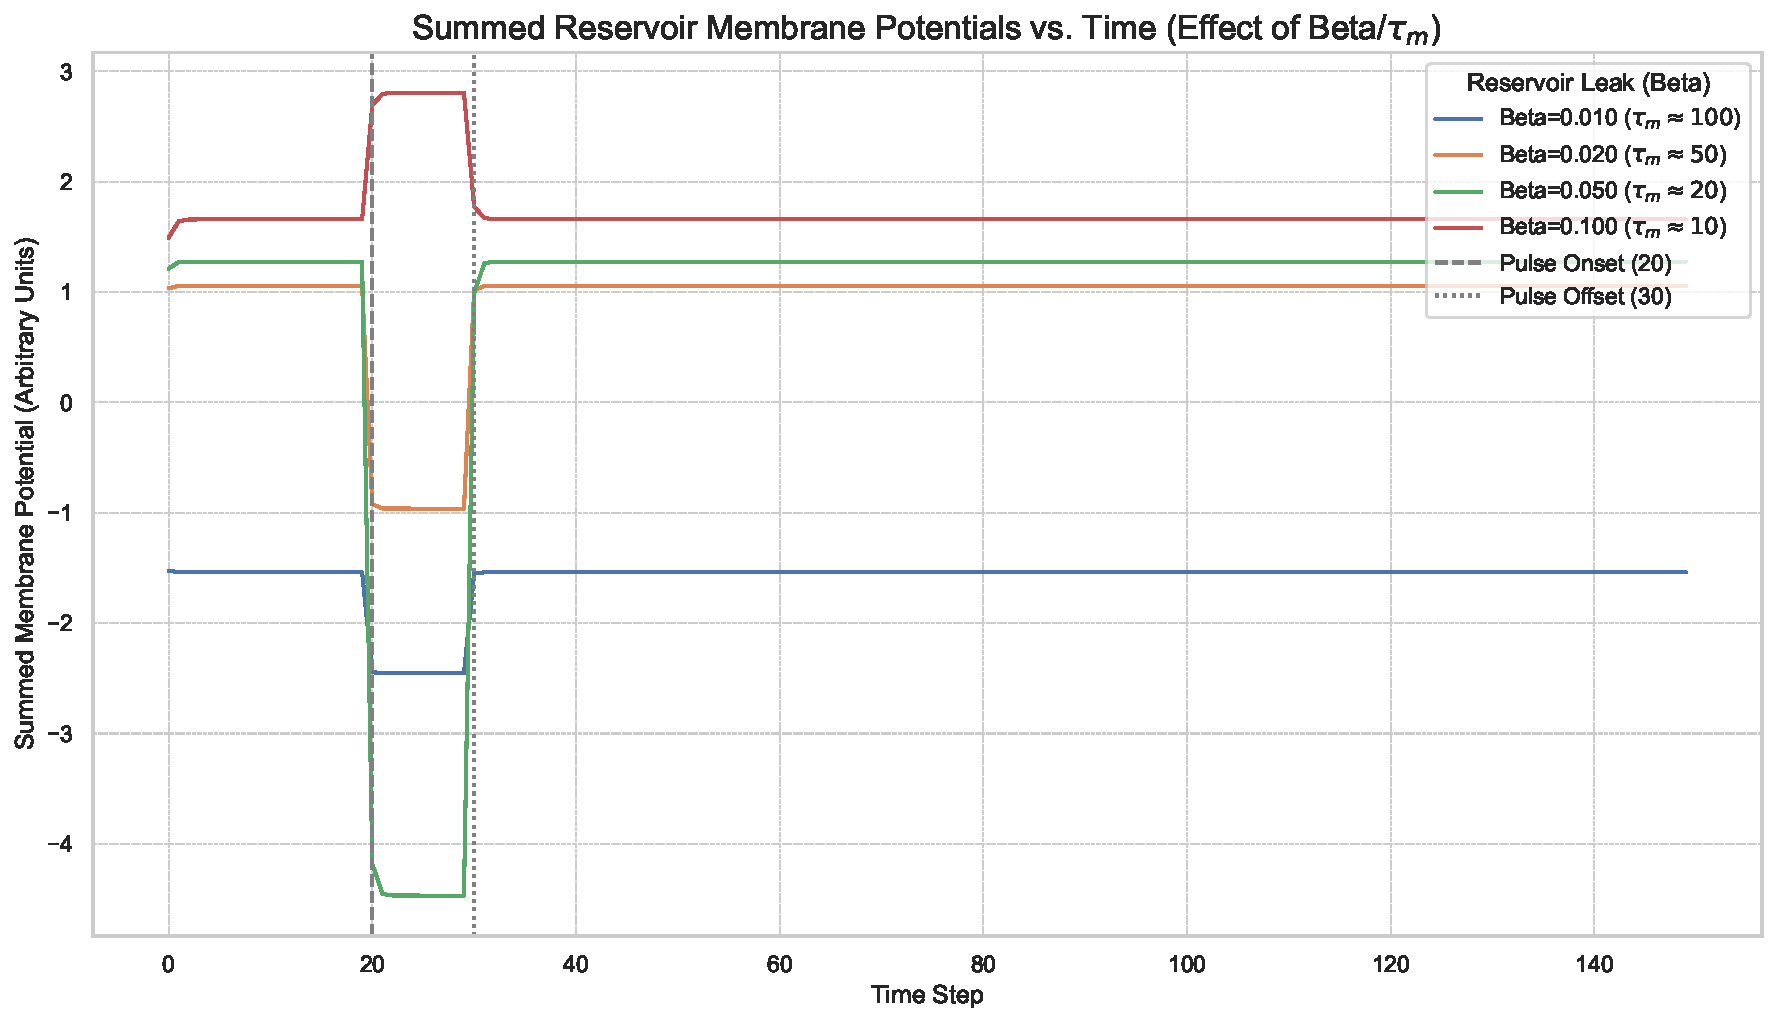
\includegraphics[width=0.9\textwidth]{pictures/chLSM/lsm_summed_activity_beta_comparison.pdf}
    \caption{Summed reservoir membrane potentials over time for different $\beta$ values. The input pulse was active from time step 20 to 30. Smaller $\beta$ (larger $\tau_m$) produces more sustained responses, consistent with first-order low-pass filtering.}
    \label{fig:summed_beta_response}
\end{figure}

\begin{figure}[H]
    \centering
    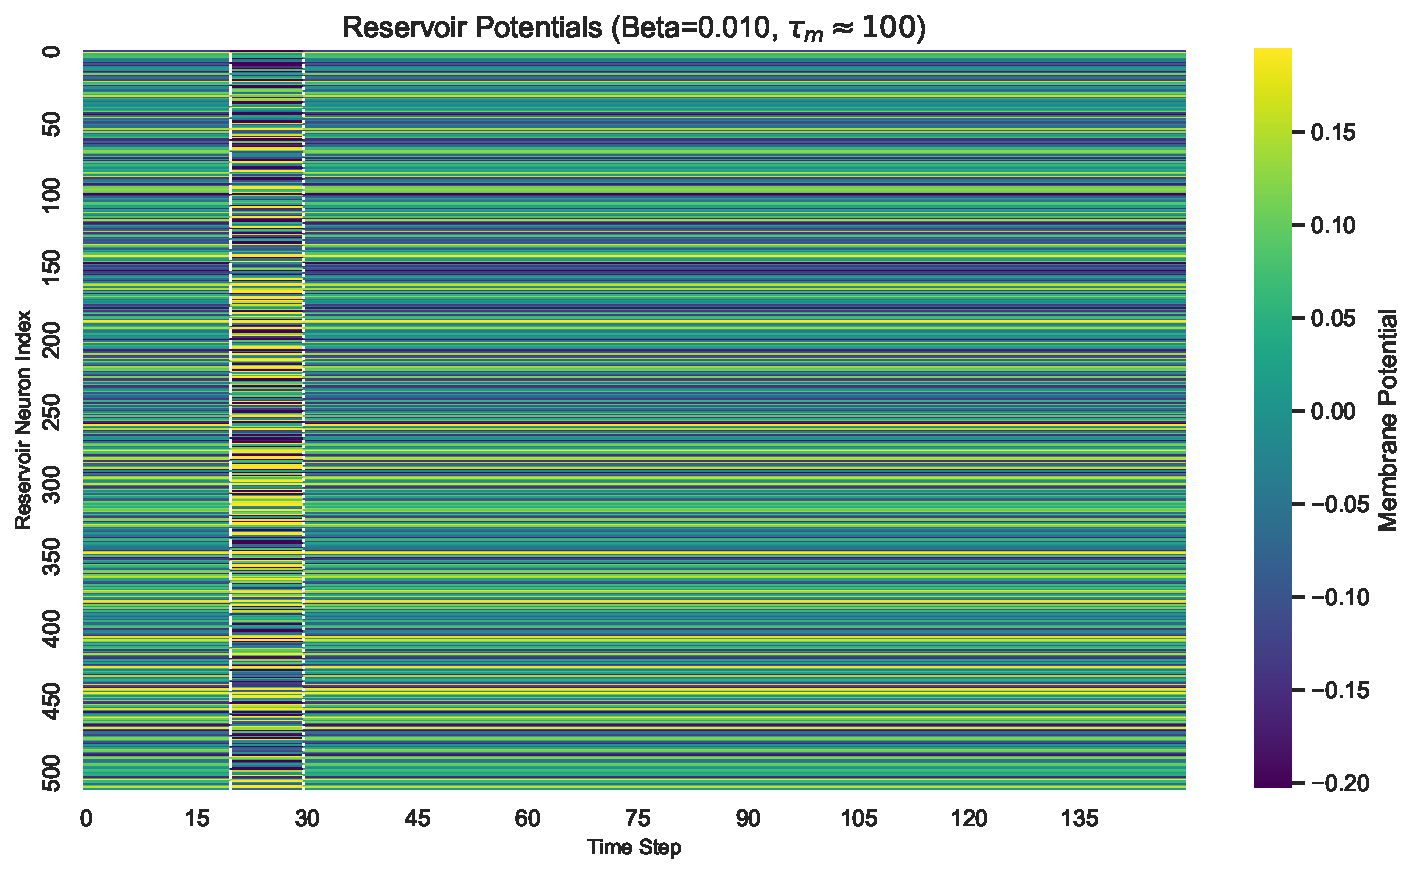
\includegraphics[width=0.8\textwidth]{pictures/chLSM/lsm_heatmap_beta_0p01.pdf}
    \caption{Heatmap of membrane potentials for all 512 reservoir neurons with $\beta = 0.010$ ($\tau_m \approx 100$). Activity is sustained across many neurons long after the input pulse, reflecting long temporal integration.}
    \label{fig:heatmap_beta_slow}
\end{figure}

\begin{figure}[H]
    \centering
    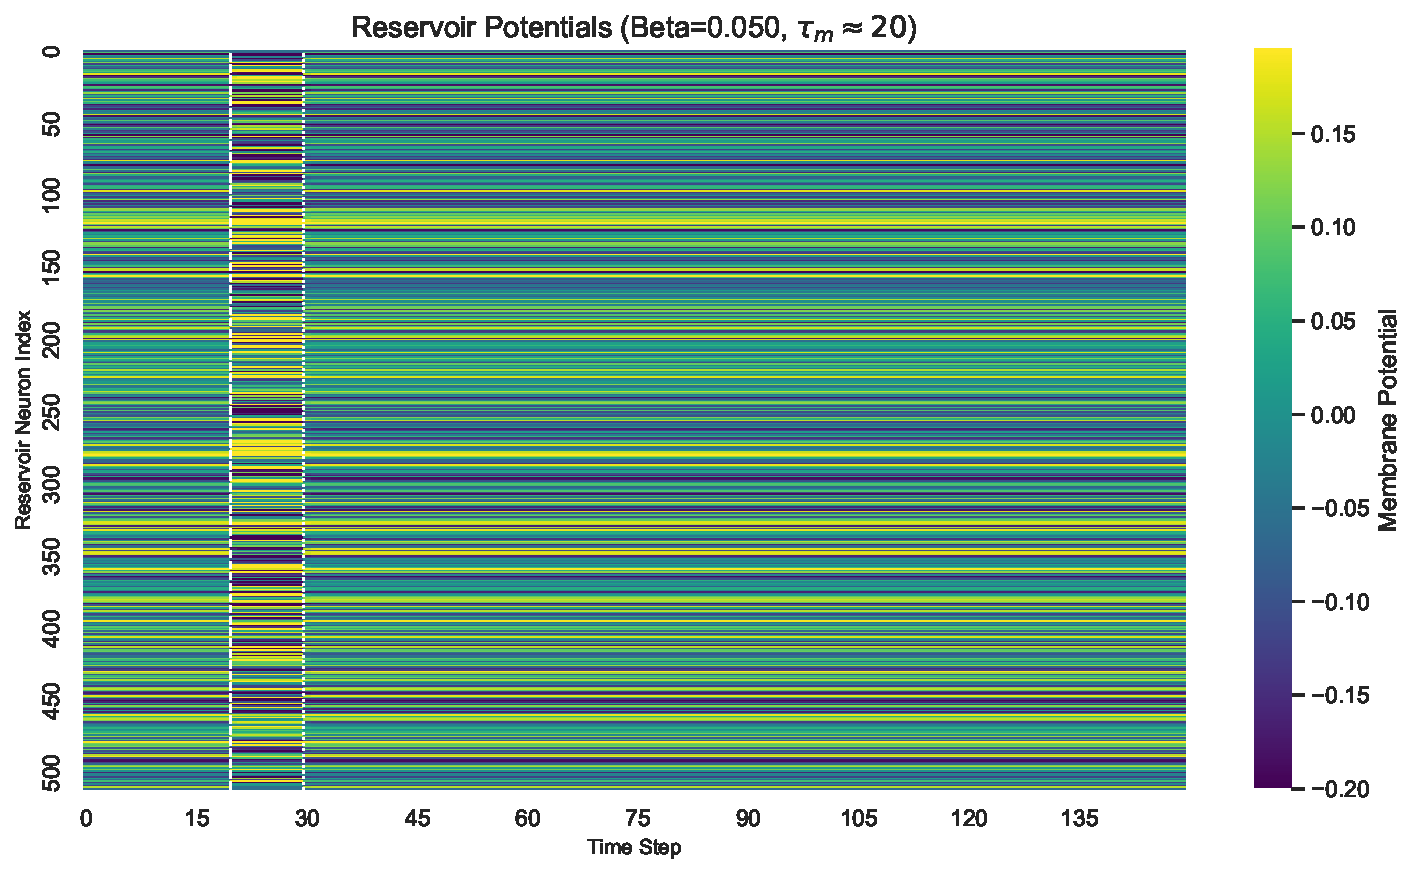
\includegraphics[width=0.8\textwidth]{pictures/chLSM/lsm_heatmap_beta_0p05.pdf}
    \caption{Heatmap of membrane potentials for all 512 reservoir neurons with $\beta = 0.050$ ($\tau_m \approx 20$). Activation is more transient, with most neurons returning to baseline within 30--40 steps of pulse offset.}
    \label{fig:heatmap_beta_fast}
\end{figure}

\subsection{Discussion and Significance}

The sweep shows that response persistence changes systematically with $\beta$ in this realization. For a single exponential decay, the remaining fraction after $k$ time constants is $e^{-k}\approx\{0.368,0.135,0.050,0.018\}$ for $k\in\{1,2,3,4\}$. The summed-potential traces are qualitatively consistent with that expectation \cite{gerstner_spiking_2002}, although the recurrent, thresholded population is not an exact single-exponential system.

The aggregate and unit-level plots are both consistent with a contribution from the decay parameter. A causal decomposition would require an ablation of recurrence or a matched analytic model, which was not performed here.

$\beta=0.05$ was retained as a provisional engineering choice because its response persisted through the immediate post-pulse interval without remaining elevated for the full simulated epoch. No mutual information, formal memory capacity, or nonlinear capacity was estimated in this module.

For the tested pulse, the $\beta=0.05$ response is concentrated near the window later sampled in Module~3. This alignment motivates, but does not independently validate, the subsequent feature window.


%% ===================================================================
%% MODULE 2
%% ===================================================================
\section{Module 2: Input Strength, Firing Threshold, and the Transition to Spiking}
\label{sec:module2}

\subsection{Theoretical Motivation}

Module~1 described temporal persistence. Module~2 asks how the observed response changes when the selected threshold does or does not permit spikes under the tested input amplitudes.

When no unit crosses threshold, the spike-dependent recurrent term is zero and the implemented update is linear apart from the nonnegative membrane floor. Different input-weight realizations can therefore give different aggregate projections of the same pulse. Such seed dependence is expected in a random-feature model and is not, by itself, evidence of instability.

Threshold crossing introduces a piecewise nonlinearity. In the implementation used here, the threshold is subtracted from the updated membrane, the result is floored at zero, and the retained membrane term is cleared on the next step for a unit that spiked. This is not a reset of every spike to one identical post-spike value, and the present design does not estimate whether it reduces seed sensitivity.

The practical criterion used here is simpler than a proof of separation or approximation: the selected configuration should emit nonzero, amplitude-dependent spikes that can be summarized by the downstream feature extractor.

This module empirically characterizes both regimes and tests which provides a more reliable basis for downstream feature extraction, a decision with direct architectural consequences for ARSPI-Net.

\subsection{Experimental Design}

Two threshold conditions were examined: $M_{\text{th}} = 1.0$ (high threshold, suppressing spiking) and $M_{\text{th}} = 0.5$ (low threshold, enabling spiking). For each condition, input pulse amplitudes of 0.6, 1.2, and 2.0 were applied (all other parameters as in Module~1, with $\beta = 0.05$). To assess initialization sensitivity in the subthreshold regime, the $M_{\text{th}} = 1.0$ condition was repeated across $N_{\text{instances}} = 5$ independent LSM instances, each with a newly initialized $\mathbf{W}^{\text{in}}$ (Xavier uniform) but identical $\mathbf{W}^{\text{rec}}$ and neuron parameters. The $M_{\text{th}} = 0.5$ condition was analyzed from a single representative instance, consistent with the exploratory objective of identifying a functional spiking regime.

Key observables included the summed membrane potential $V_{\text{summed}}[t]$ (Equation~\ref{eq:v_summed}), the instantaneous population firing rate $R[t] = (1/N_{\text{res}}) \sum_i S_i[t]$, the total spike count during the pulse window (steps 20--30), and the peak population firing rate.

\subsection{Results: Subthreshold Regime \texorpdfstring{($M_{\text{th}} = 1.0$)}{(threshold = 1.0)}}
\label{sec:subthreshold_results}

Across the five high-threshold input-weight realizations, the aggregate membrane summaries varied visibly. Peak deflection was non-monotonic in one realization, decreased with amplitude in two, showed a plateau followed by a change in one, and was nearly flat in one (Figures~\ref{fig:instance1_thresh1_standalone}--\ref{fig:instance5_thresh1_standalone}). Figure~\ref{fig:summary_thresh1_new} summarizes these five descriptive observations; with only five realizations, it is not a population estimate of seed robustness.

Each $\mathbf{W}^{\text{in}}$ realization defines a different random projection, so seed-dependent aggregate responses are unsurprising \cite{Norton2020_NextGenRC,Lukosevicius2009_Reservoir}. The observed input--summary relationship is therefore a property of both the stated architecture and its realized weights.

\begin{figure}[H]
    \centering
    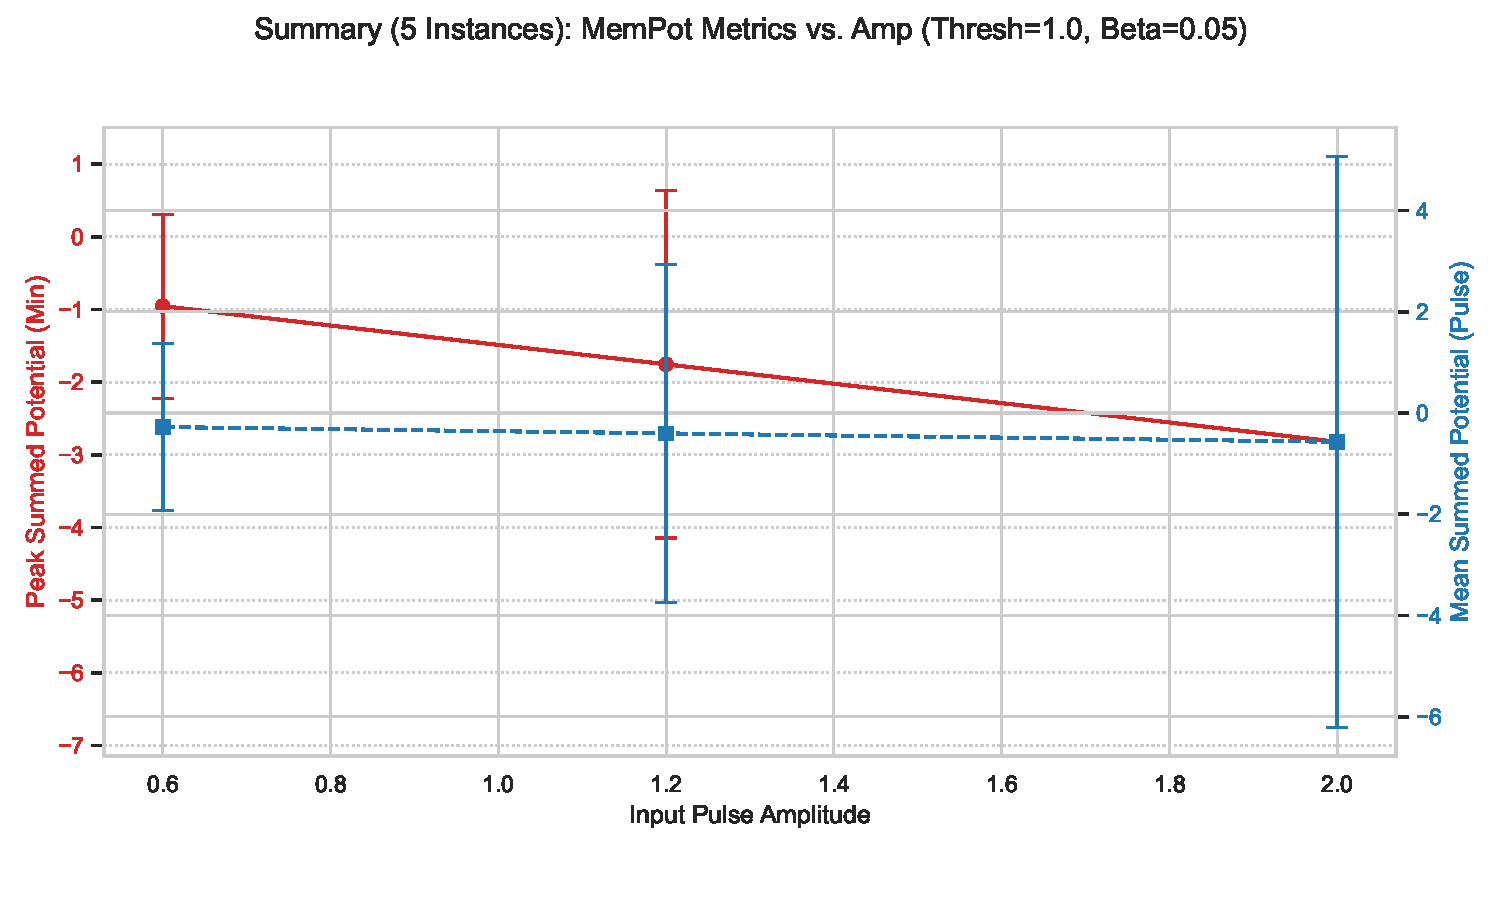
\includegraphics[width=0.7\textwidth]{pictures/chLSM/summary_mempot_metrics_thresh1p0.pdf}
    \caption{Summary of subthreshold metrics versus input amplitude across 5 network instances ($M_{\text{th}} = 1.0$, $\beta = 0.05$). Error bars represent standard deviation. The large variability reflects the sensitivity of continuous-valued trajectories to the random input projection.}
    \label{fig:summary_thresh1_new}
\end{figure}

\begin{figure}[H]
    \centering
    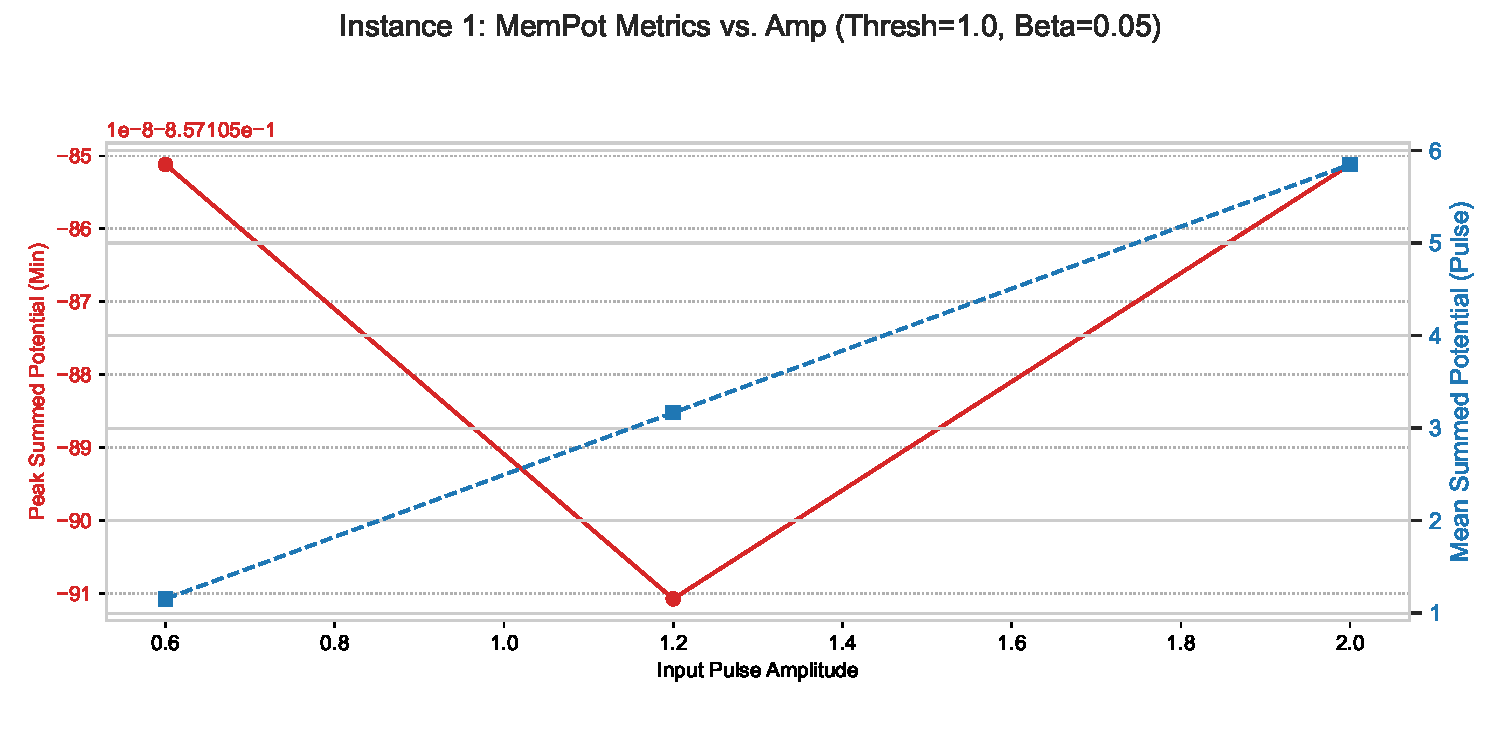
\includegraphics[width=0.7\textwidth]{pictures/chLSM/instance1_mempot_metrics_thresh1p0.pdf}
    \caption{Instance 1: Non-monotonic peak deflection, monotonically increasing mean potential.}
    \label{fig:instance1_thresh1_standalone}
\end{figure}

\begin{figure}[H]
    \centering
    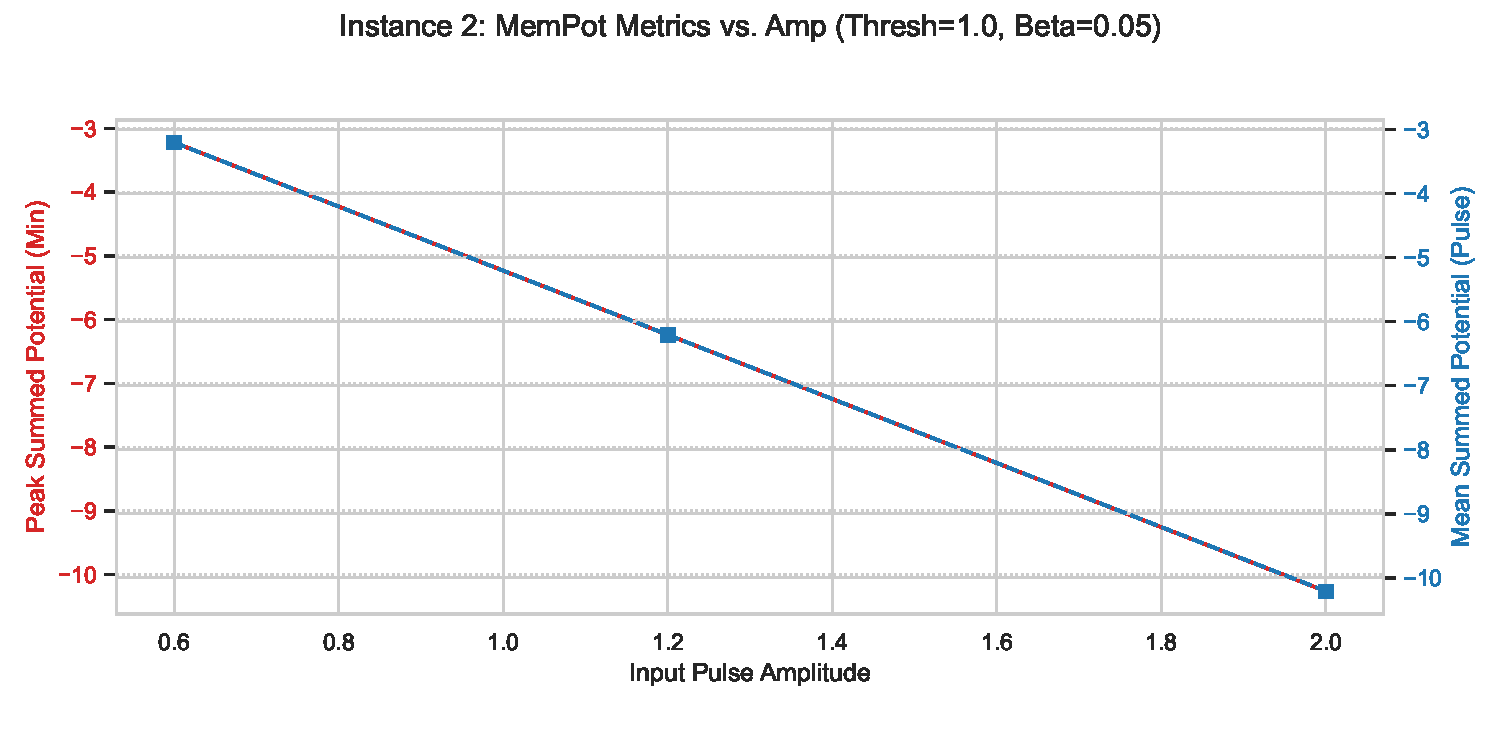
\includegraphics[width=0.7\textwidth]{pictures/chLSM/instance2_mempot_metrics_thresh1p0.pdf}
    \caption{Instance 2: Both metrics show strong monotonic decrease with input amplitude.}
    \label{fig:instance2_thresh1_standalone}
\end{figure}

\begin{figure}[H]
    \centering
    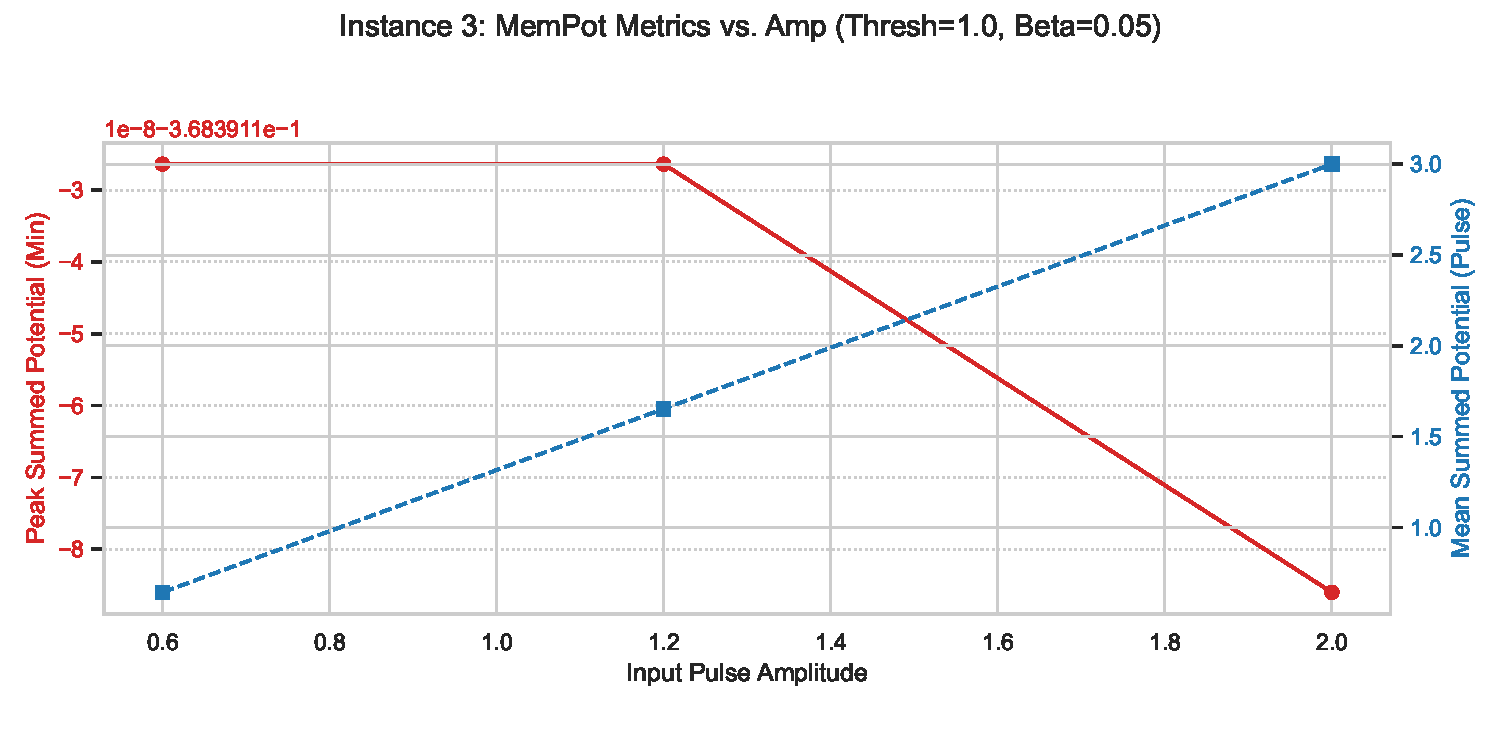
\includegraphics[width=0.7\textwidth]{pictures/chLSM/instance3_mempot_metrics_thresh1p0.pdf}
    \caption{Instance 3: Plateau followed by sharp decrease; monotonically increasing mean.}
    \label{fig:instance3_thresh1_standalone}
\end{figure}

\begin{figure}[H]
    \centering
    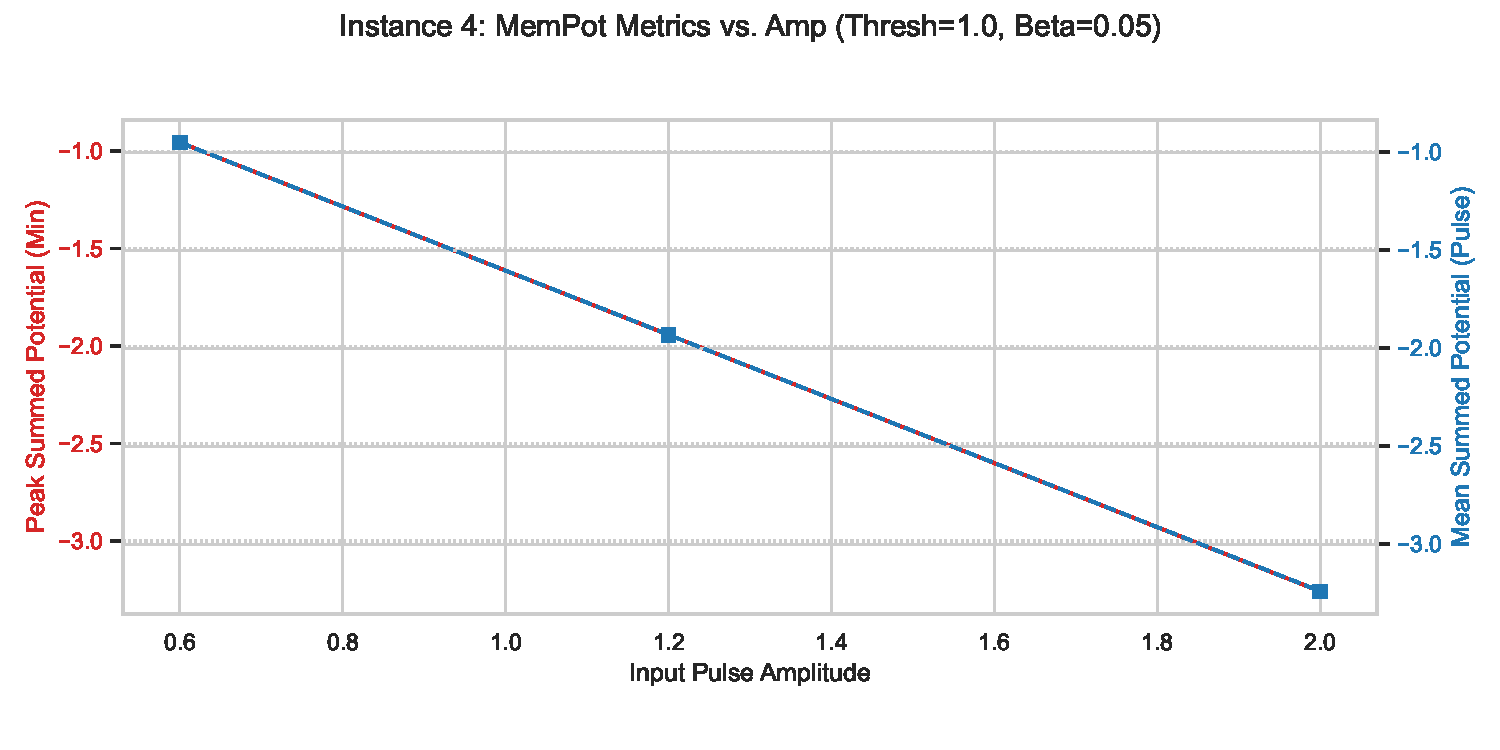
\includegraphics[width=0.7\textwidth]{pictures/chLSM/instance4_mempot_metrics_thresh1p0.pdf}
    \caption{Instance 4: Consistent monotonic decrease, similar to Instance 2.}
    \label{fig:instance4_thresh1_standalone}
\end{figure}

\begin{figure}[H]
    \centering
    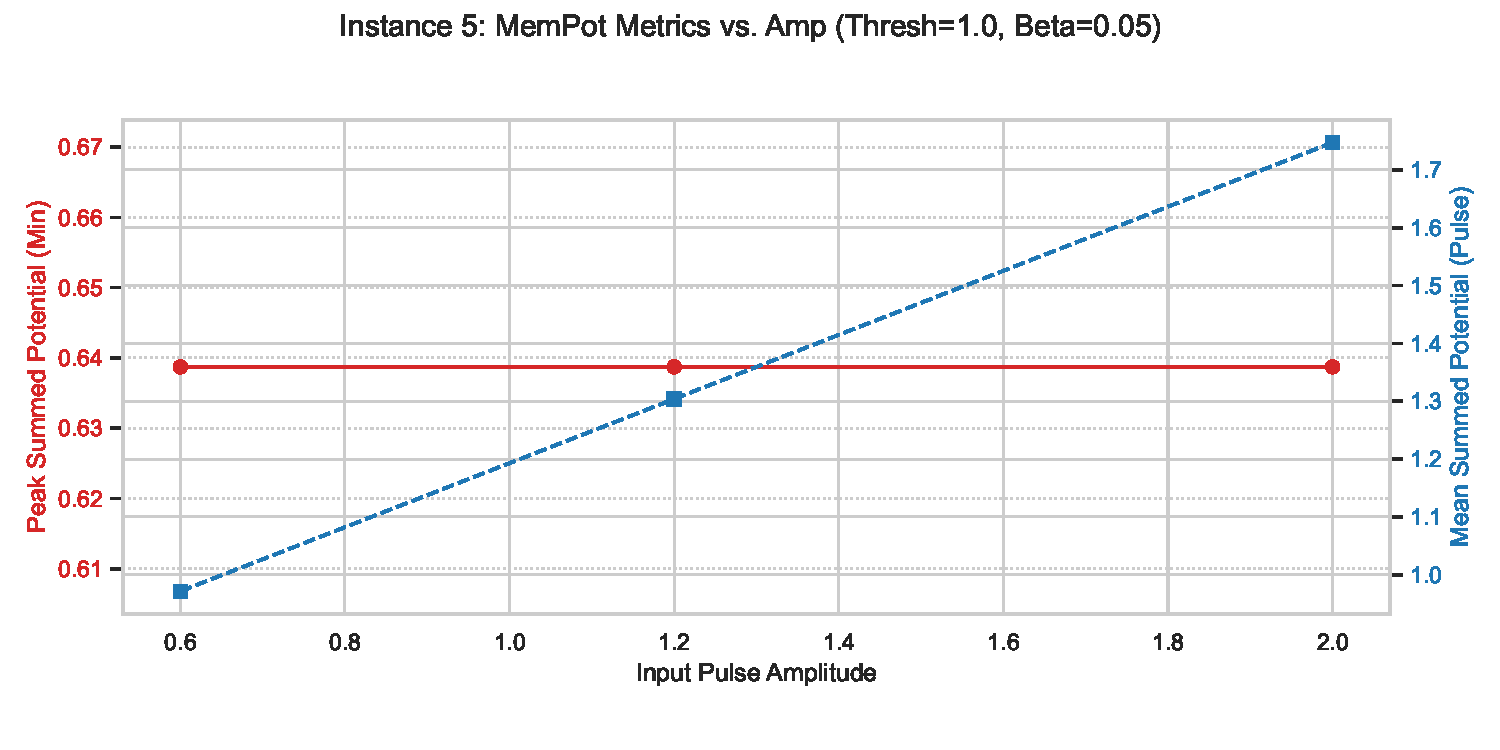
\includegraphics[width=0.7\textwidth]{pictures/chLSM/instance5_mempot_metrics_thresh1p0.pdf}
    \caption{Instance 5: Nearly constant peak deflection; monotonically increasing mean.}
    \label{fig:instance5_thresh1_standalone}
\end{figure}

\subsection{Results: Spiking Regime \texorpdfstring{($M_{\text{th}} = 0.5$)}{(threshold = 0.5)}}
\label{sec:spiking_results}

In the one low-threshold realization examined, lowering $M_{\text{th}}$ to 0.5 produced spike activity that increased with input amplitude. Because this condition was not repeated across seeds, the result does not establish robustness or reproducibility across initializations.

The archived summed-potential figure (Figure~\ref{fig:m2_summed_mempot_thresh0p5_actual}) has positive deflections at amplitudes 0.6 and 1.2 and negative values at amplitude 2.0 during the pulse. Because the audited implementation floors each retained membrane value at zero, this sign change cannot be attributed to that implementation. Figure~\ref{fig:m2_mempot_metrics_thresh0p5_actual} is retained only to document the legacy run.

In the archived firing-rate figure (Figure~\ref{fig:m2_pop_firing_rate_thresh0p5_actual}), amplitude 0.6 produces almost no spikes, amplitude 1.2 produces about five spikes during the pulse, and amplitude 2.0 produces about 170. This is an amplitude ordering in one legacy realization, not a calibrated population frequency--current curve or a cross-seed result.

\begin{figure}[H]
    \centering
    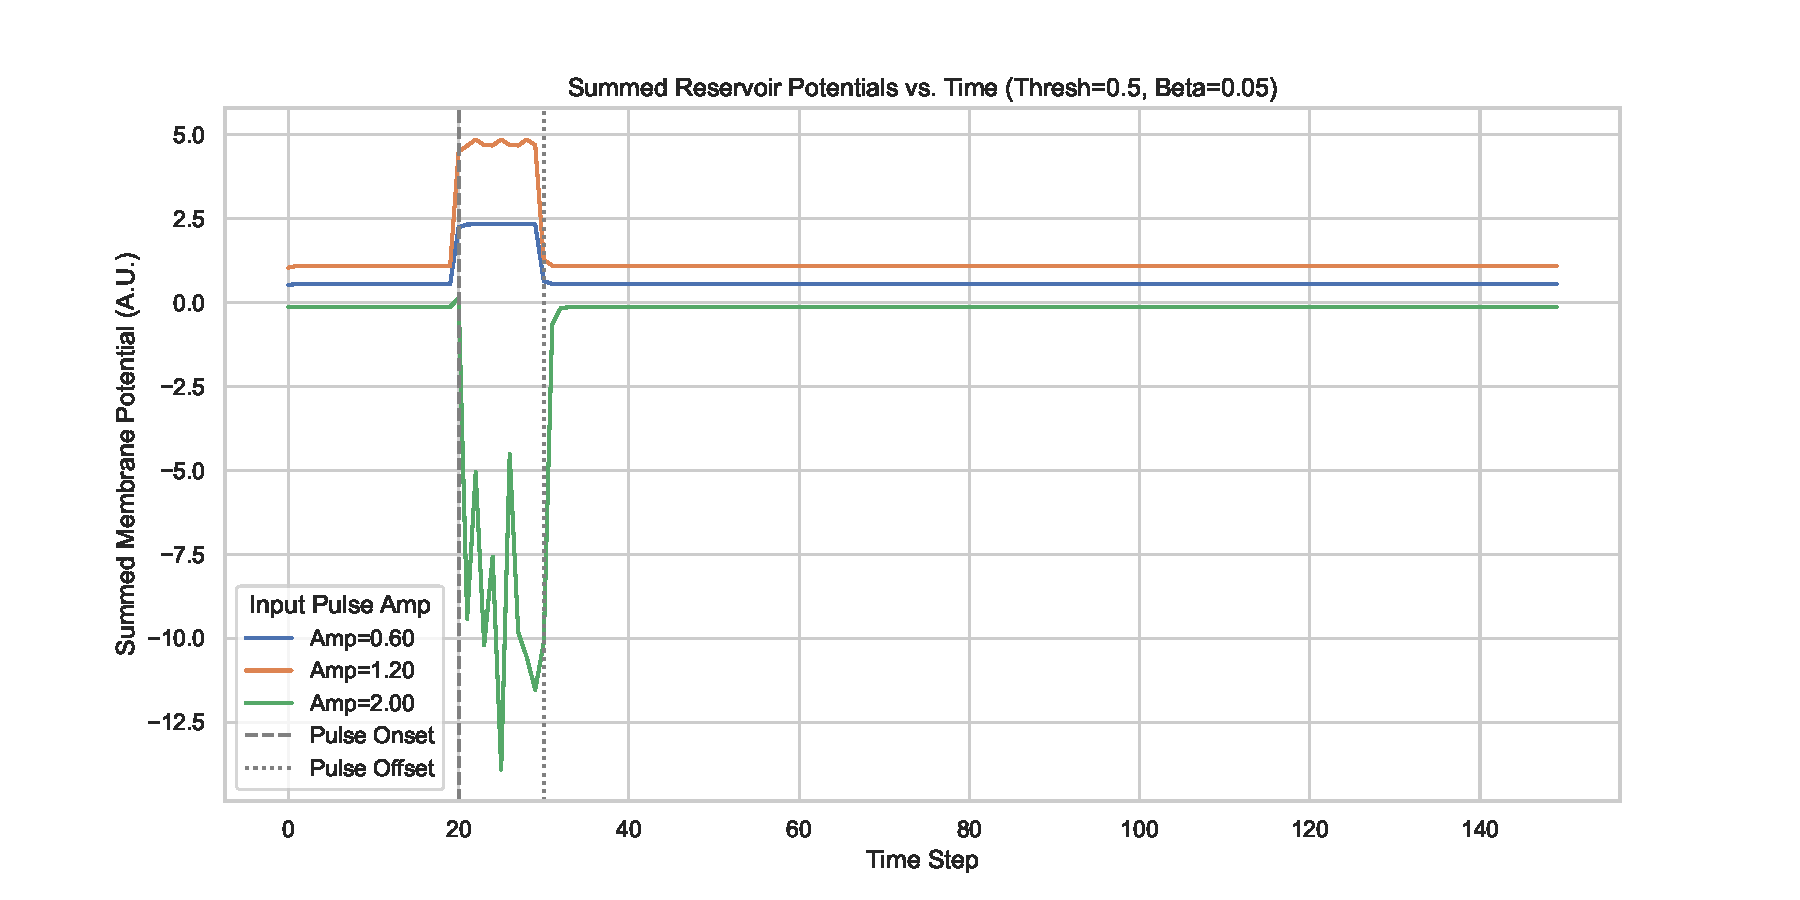
\includegraphics[width=0.9\textwidth]{pictures/chLSM/summed_mempot_thresh0p5.pdf}
    \caption{Archived summed membrane potentials in the low-threshold run ($M_{\text{th}} = 0.5$, $\beta = 0.05$). The negative retained values are incompatible with the audited nonnegative-floor update, so the plot is a legacy observation rather than current-model verification.}
    \label{fig:m2_summed_mempot_thresh0p5_actual}
\end{figure}

\begin{figure}[H]
    \centering
    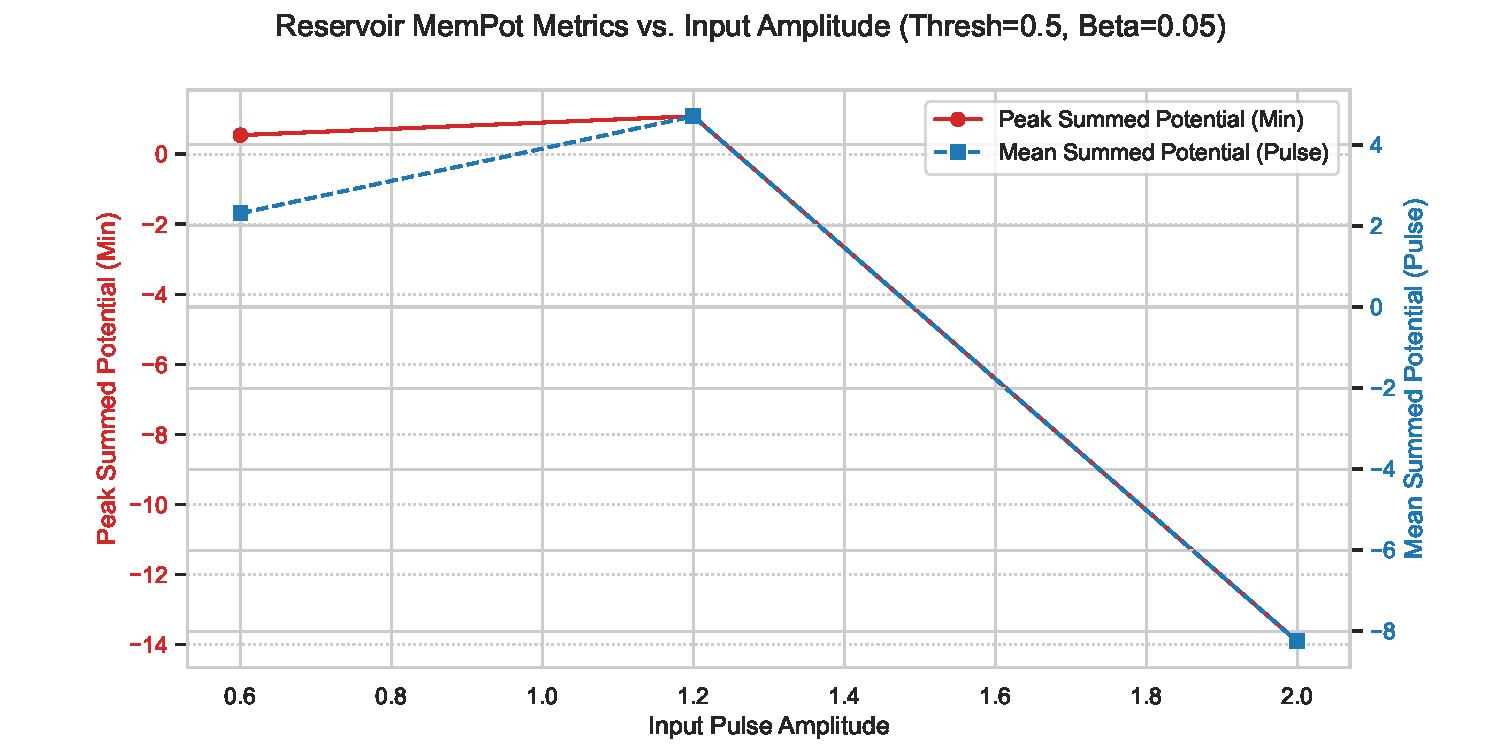
\includegraphics[width=0.8\textwidth]{pictures/chLSM/mempot_metrics_vs_amp_thresh0p5.pdf}
    \caption{Archived membrane summaries versus input amplitude in the low-threshold run. The sign change at the largest amplitude inherits the legacy-update mismatch.}
    \label{fig:m2_mempot_metrics_thresh0p5_actual}
\end{figure}

\begin{figure}[H]
    \centering
    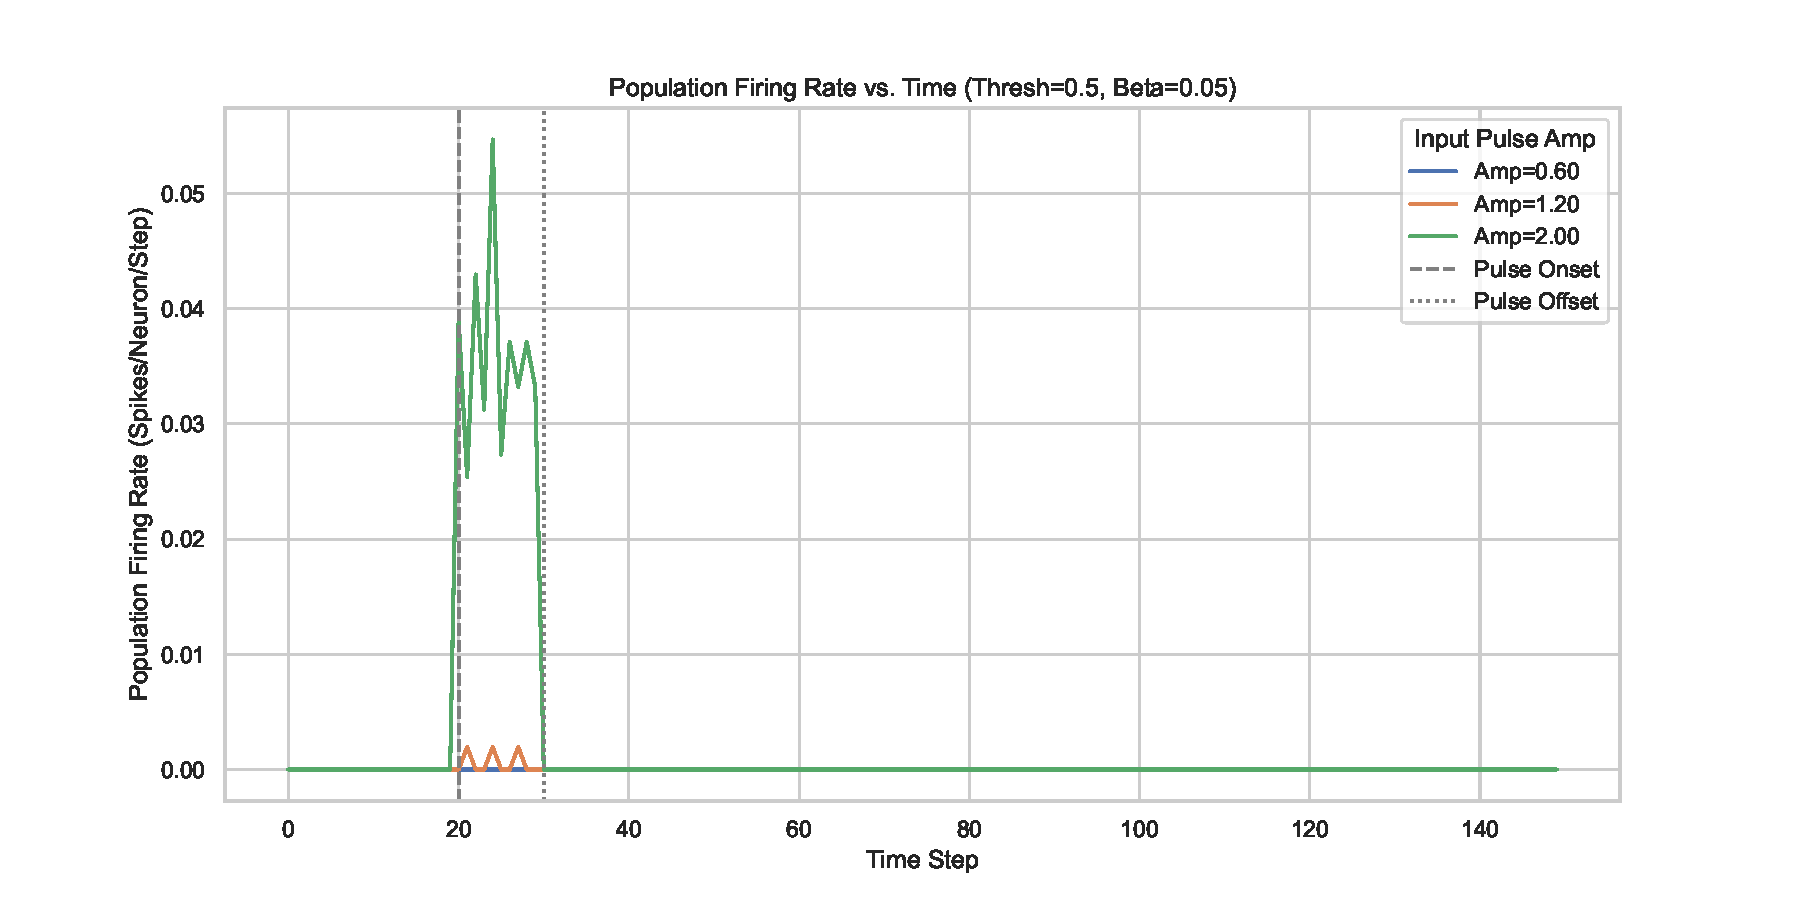
\includegraphics[width=0.9\textwidth]{pictures/chLSM/pop_firing_rate_thresh0p5.pdf}
    \caption{Population firing rate versus time for three input amplitudes in one reservoir realization ($M_{\text{th}}=0.5$, $\beta=0.05$). Spiking increased with input strength in this realization.}
    \label{fig:m2_pop_firing_rate_thresh0p5_actual}
\end{figure}

\begin{figure}[H]
    \centering
    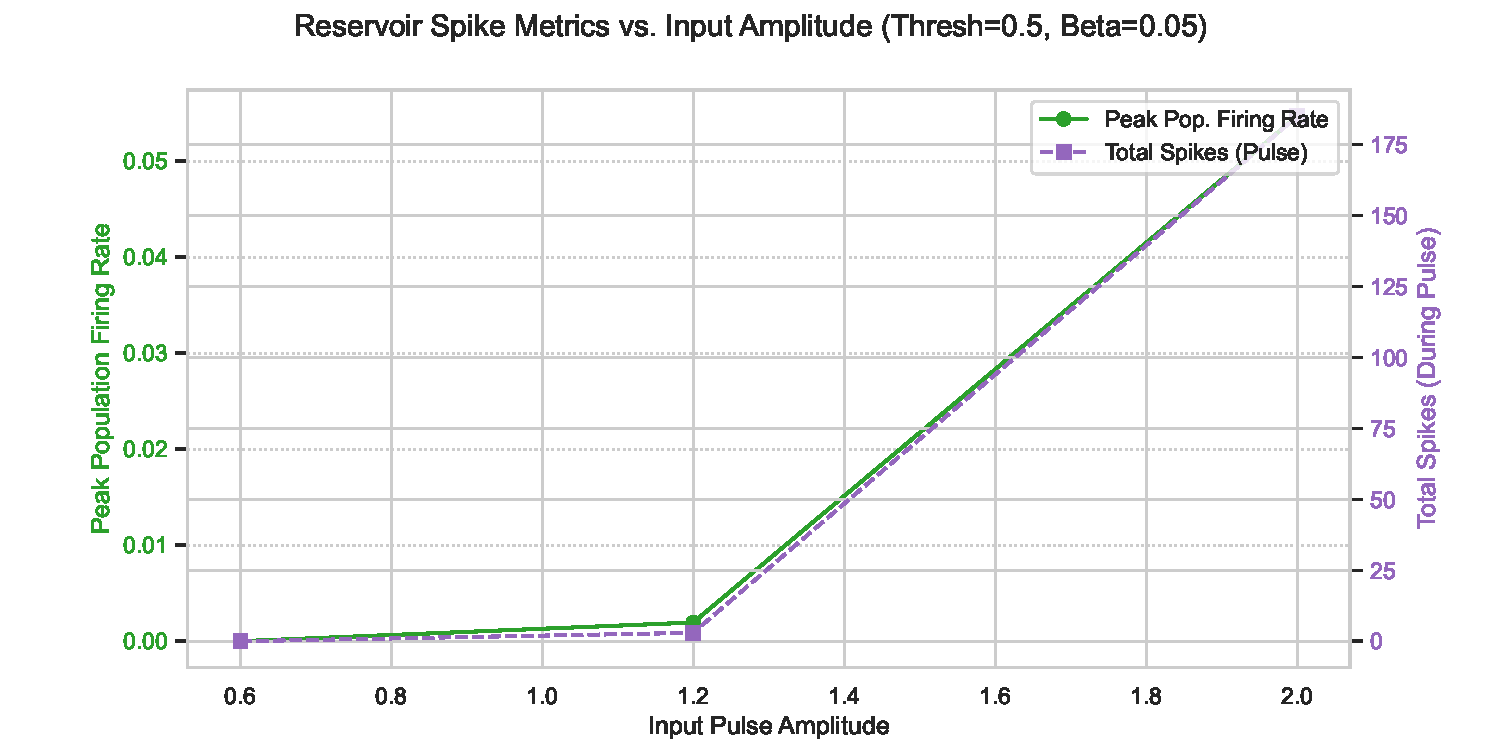
\includegraphics[width=0.8\textwidth]{pictures/chLSM/spike_metrics_vs_amp_thresh0p5.pdf}
    \caption{Archived peak population firing rate and total spike count versus input amplitude in one realization. The three points show an amplitude ordering but do not estimate a population frequency--current curve.}
    \label{fig:m2_spike_metrics_thresh0p5_actual}
\end{figure}

\subsection{Discussion and Significance}
\label{sec:module2_discussion}

The module documents different response summaries under the two threshold settings, while its asymmetric seed sampling limits between-regime inference.

\subsubsection{The Regularizing Role of the Spiking Nonlinearity}

The high-threshold plots show that aggregate membrane summaries depend on the random projection. This does not make the regime intrinsically unreliable: random-feature systems are normally calibrated with their realized weights. It does mean that the summaries should not be presented as architecture-only quantities.

The low-threshold update adds thresholding and reset to the response, producing a nonlinear spike-count feature. A matched multi-seed experiment would be needed to determine whether that feature is more consistent across realizations than the high-threshold membrane summaries.

\subsubsection{The Population Rate Code and Its Engineering Significance}

Continuous-time LIF models have a monotonic frequency--current relationship above threshold \cite{gerstner_spiking_2002,dayan2001}. The custom discrete update here is not identical to that analytic model, but the observed increase in total spikes and peak population rate with amplitude is qualitatively consistent with it. Spike counts are therefore retained as candidate downstream features.

The population firing-rate vector $\mathbf{r}=[r_1,\ldots,r_{N_{\text{res}}}]$ is a high-dimensional summary whose components reflect different input and recurrent weights. The tested amplitude sweep shows that this summary is nonconstant and graded in the selected realization; it does not quantify how much input information is preserved.

Robust spike coding has been demonstrated for networks designed around coordinated error correction \cite{Boerlin2013_PredictiveCoding}. The present random reservoir does not implement that construction, so the citation supplies context rather than evidence that this reservoir has the same robustness property.

\subsubsection{Implications for ARSPI-Net}

The threshold $M_{\text{th}}=0.5$ was adopted provisionally because it produced a nonzero, amplitude-dependent spike code in the selected realization and is compatible with binned spike-count features. Cross-seed superiority over the high-threshold setting remains untested in this module.


%% ===================================================================
%% MODULE 3
%% ===================================================================
\section{Module 3: Temporal Localization of Discriminative Information}
\label{sec:module3}

\subsection{Theoretical Motivation}

Modules~1 and 2 produced provisional temporal and threshold settings. The next question is which tested window yields distinct mean firing-rate vectors for the two synthetic responses.

Mean firing rate discards within-window timing and correlations, so failure of this readout would not prove that the full state is identical. No mutual information is estimated in this module.

The single-unit decay approximation suggests that an early window may retain a larger pulse response than a late window, while recurrence can alter that pattern. The experiment compares readout summaries; it does not prove that the full reservoir has fading memory or determine whether sustained recurrent patterns exist.

The comparison provides one input to window selection. With only four prespecified windows and two unique signals, it cannot identify an optimal window or estimate memory capacity.

\subsection{Experimental Design}

A binary deterministic contrast was defined: Class~0 (pulse amplitude 1.2) versus Class~1 (pulse amplitude 2.0). The generator introduced no noise, jitter, or other within-class variation, so the 200 stored rows per class were repeated copies of one class-specific response rather than independent trials. The effective number of unique input signals was therefore two. Mean firing rates from the 512-unit response were extracted from four temporal windows:
\begin{itemize}
    \item \textbf{Early Window}: time steps 20--50 (stimulus onset plus 20 post-stimulus steps)
    \item \textbf{Late Window}: time steps 50--100
    \item \textbf{Full Response Window}: time steps 20--150
    \item \textbf{Entire Trial}: time steps 0--150
\end{itemize}
Each window produced a 512-dimensional feature vector per stored row. Logistic regression with L2 regularization ($C=0.1$) was evaluated using five stratified folds, with \texttt{StandardScaler} fitted on each training fold. Because identical rows occur in both training and test folds, these scores are a deterministic separability check and must not be interpreted as independent out-of-sample validation.

\subsection{Results}

For the two unique responses, the Early Window, Full Response Window, and Entire Trial feature vectors were separable by the fitted readout (reported fold accuracy $1.000\pm0.000$), whereas the Late Window vectors were not distinguished (reported accuracy $0.500\pm0.000$; Figure~\ref{fig:m3_accuracy_cv_comparison}). The zero fold variance is expected from duplicated deterministic rows and is not a precision estimate.

The confusion matrices in Figure~\ref{fig:m3_confusion_matrices_cv} count stored duplicates, not 400 independent observations. They show that the classifier assigned all duplicates correctly when the early response was included and assigned all Late Window duplicates to Class~0 when the two late feature vectors were not distinguished by this readout.

\begin{figure}[H]
    \centering
    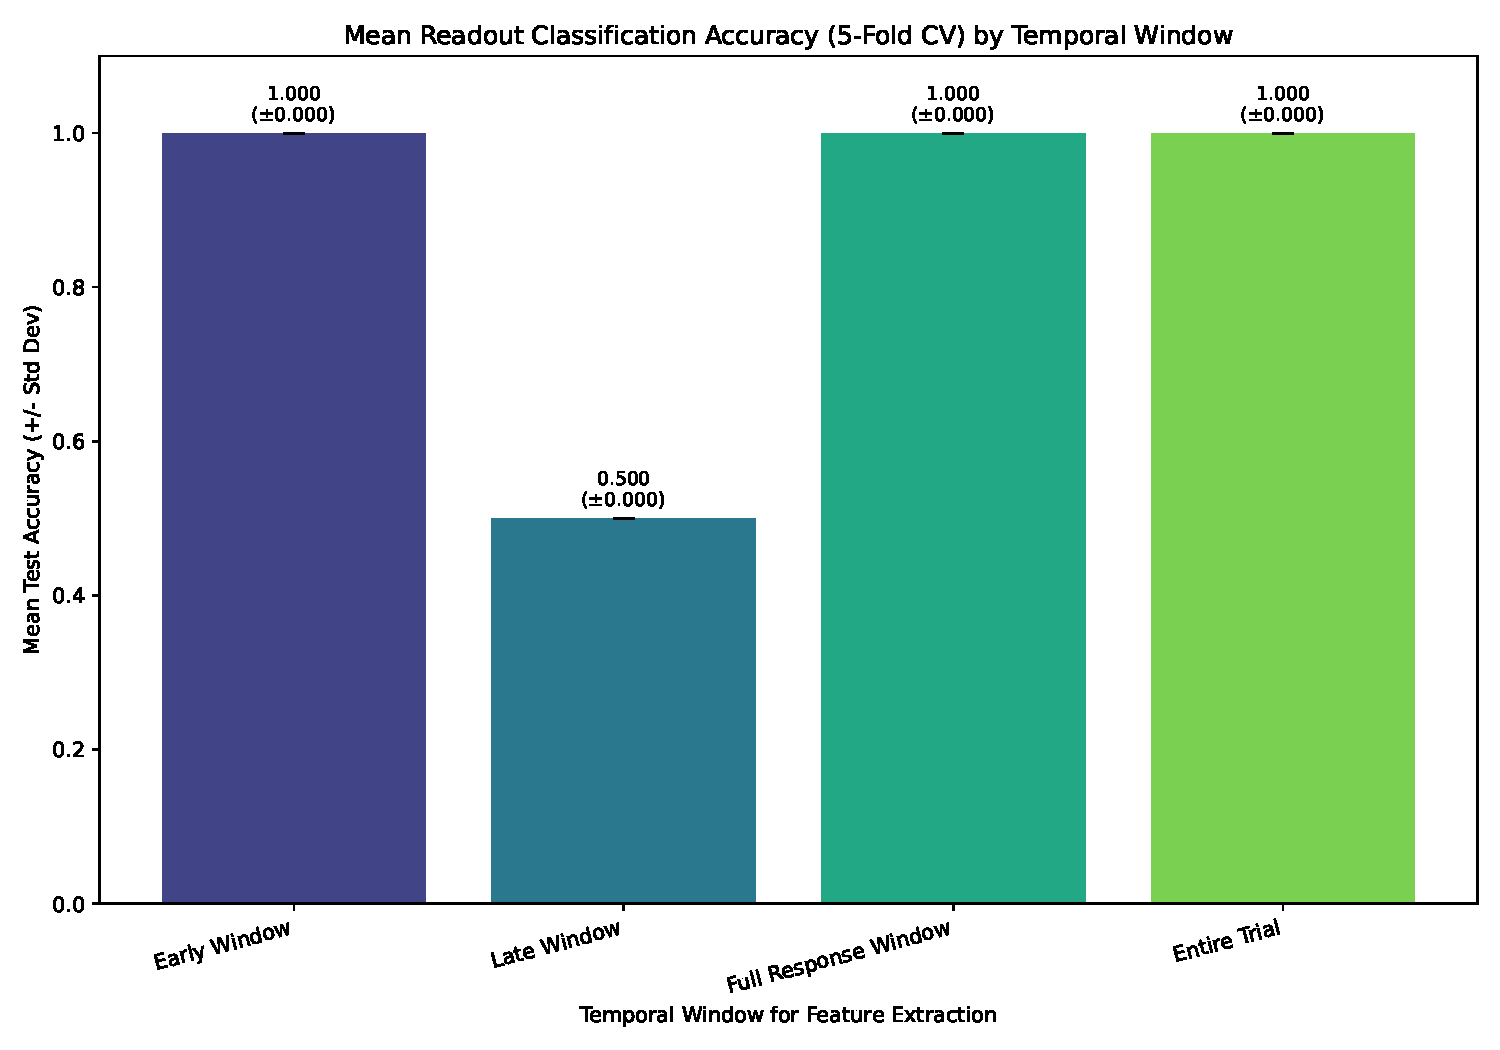
\includegraphics[width=0.9\textwidth]{pictures/chLSM/readout_accuracy_cv_comparison.pdf}
    \caption{Reported five-fold accuracy for readouts trained on deterministic, duplicated feature rows. The two unique class responses were separable when the early response was included but not from the Late Window mean rates. These are separability checks, not independent generalization estimates.}
    \label{fig:m3_accuracy_cv_comparison}
\end{figure}

\begin{figure}[H]
    \centering
    \begin{subfigure}{0.48\textwidth}
        \centering
        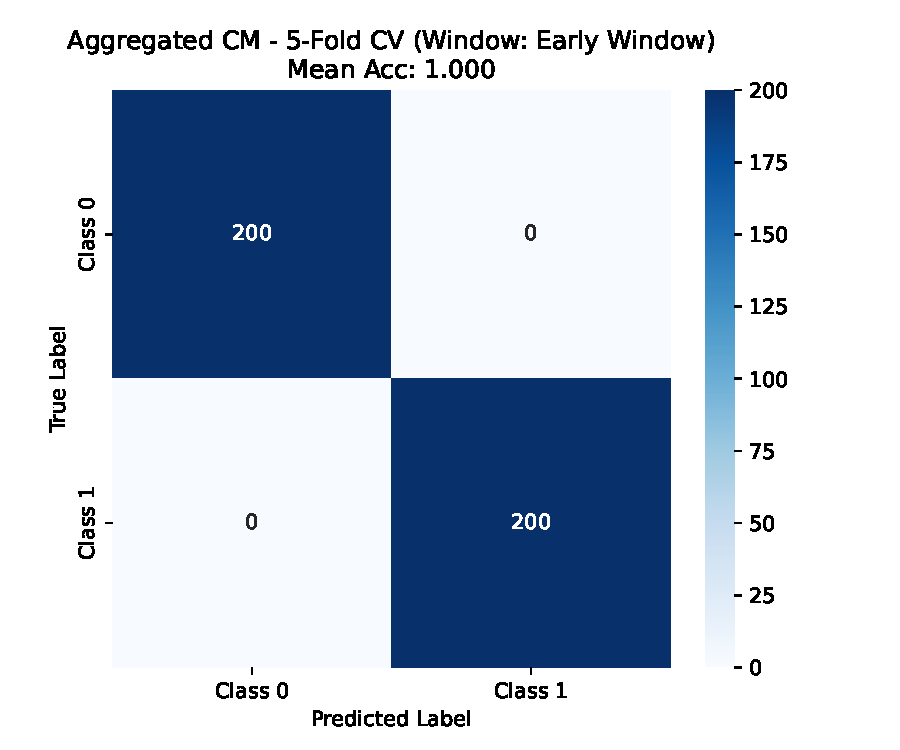
\includegraphics[width=\linewidth]{pictures/chLSM/confusion_matrix_cv_window_early_window.pdf}
        \caption{Early Window (Acc: 1.000)}
        \label{fig:m3_cm_cv_early}
    \end{subfigure}
    \hfill
    \begin{subfigure}{0.48\textwidth}
        \centering
        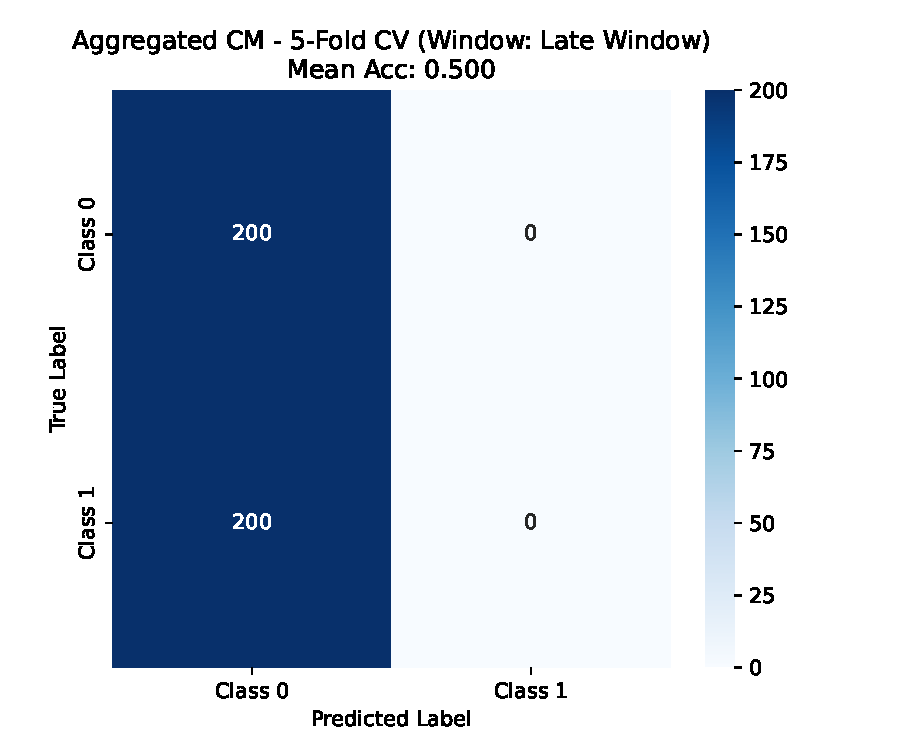
\includegraphics[width=\linewidth]{pictures/chLSM/confusion_matrix_cv_window_late_window.pdf}
        \caption{Late Window (Acc: 0.500)}
        \label{fig:m3_cm_cv_late}
    \end{subfigure}
    \vspace{1em}
    \begin{subfigure}{0.48\textwidth}
        \centering
        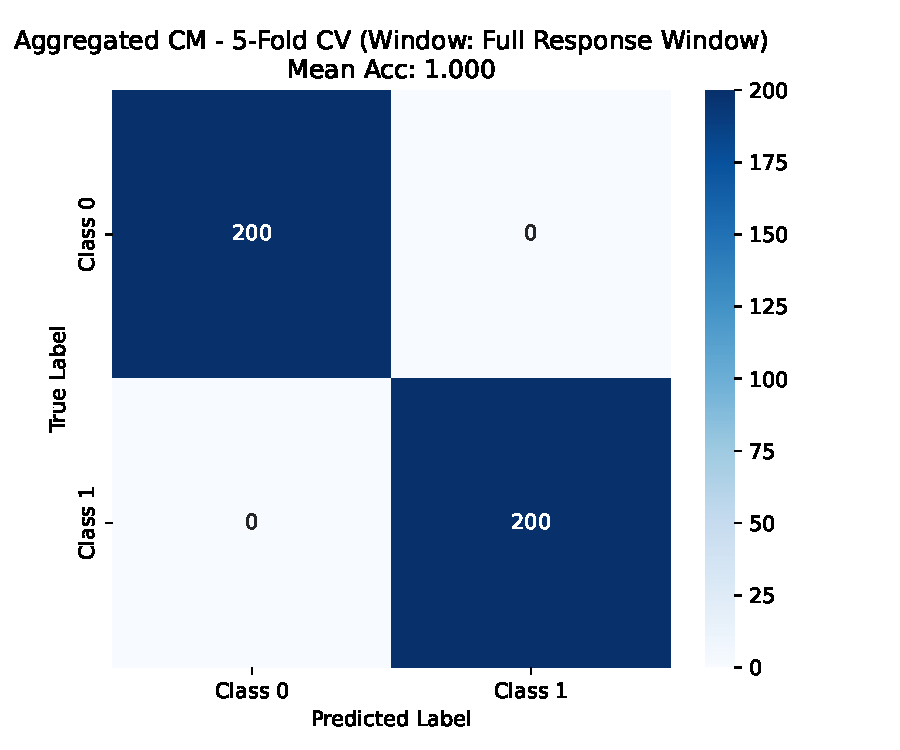
\includegraphics[width=\linewidth]{pictures/chLSM/confusion_matrix_cv_window_full_response_window.pdf}
        \caption{Full Response Window (Acc: 1.000)}
        \label{fig:m3_cm_cv_full}
    \end{subfigure}
    \hfill
    \begin{subfigure}{0.48\textwidth}
        \centering
        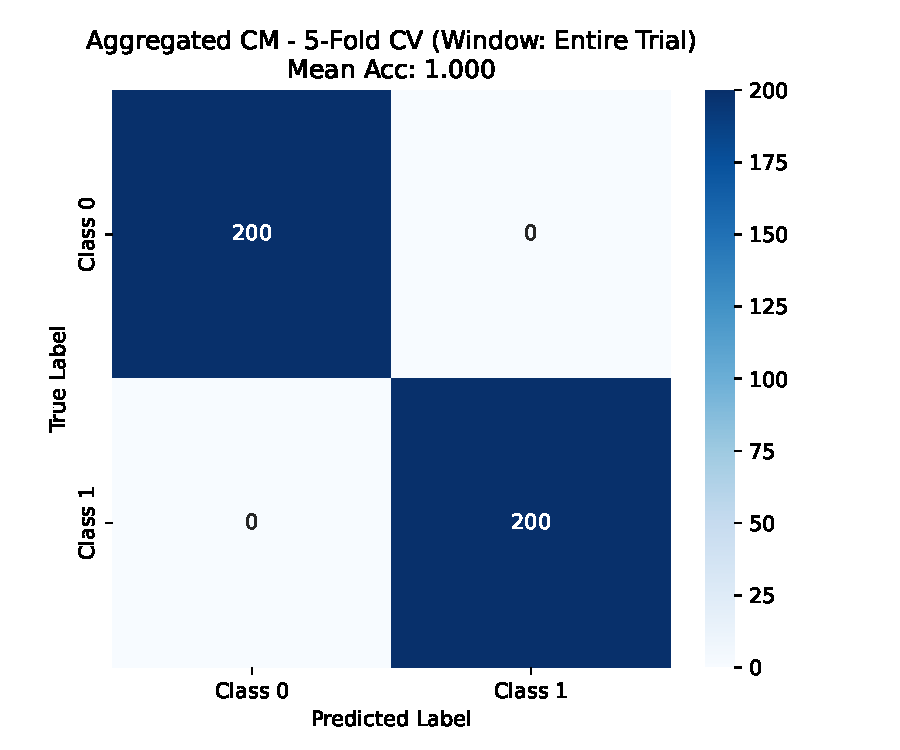
\includegraphics[width=\linewidth]{pictures/chLSM/confusion_matrix_cv_window_entire_trial.pdf}
        \caption{Entire Trial (Acc: 1.000)}
        \label{fig:m3_cm_cv_entire}
    \end{subfigure}
    \caption{Aggregated confusion matrices across five folds. Counts reflect duplicated deterministic rows (200 copies per class), not independent trials. $\beta=0.05$, $M_{\text{th}}=0.5$.}
    \label{fig:m3_confusion_matrices_cv}
\end{figure}

\subsection{Discussion and Significance}

\subsubsection{The Biophysical Basis of Information Decay}

The Late Window result is consistent with fading memory. Under a single-unit exponential approximation with $\beta=0.05$ ($\tau_m\approx20$ steps), a perturbation would fall to about 36.8\% after one time constant and about 3\% after 3.5 time constants. The classifier result alone does not establish that this mechanism caused the loss of separability in the full recurrent system.

After external drive ceases, activity reflects both decay and autonomous recurrent dynamics \cite{Sussillo2009,Barak2017}. In this realization the 50-step mean-rate readout did not distinguish the two late responses. The experiment did not identify a common attractor or test whether fine spike timing retained class structure.

\subsubsection{What Information Decay Does and Does Not Imply}

Two scope considerations qualify this finding, and both have direct consequences for the embedding pipeline developed in the next chapter.

First, the Late Window result implies only that this mean-rate readout did not distinguish the two stored vectors. Mean rate collapses within-window timing, so temporally resolved counts are a reasonable feature to test next; the result does not show that those counts will recover late structure.

Second, all units share $\beta=0.05$. Heterogeneous time constants can enrich recurrent dynamics in other settings \cite{Kim2024NeuralHeterogeneity}, but their effect on this task was not tested and remains future work.

\subsubsection{Implications for the Reservoir's Role in ARSPI-Net}

The practical observation is that temporal windowing changes this readout. For these two deterministic responses, the Early Window separated the classes and the Late Window did not. Chapter~\ref{chap:embeddings} evaluates a broader steps 10--70 window with temporally resolved coding; that later choice is not validated by the duplicate-row cross-validation here.

For this pulse family, the selected reservoir behaves as a transient transformation whose mean-rate contrast is clearest near the driven response. That limited observation motivates temporal binning but does not establish a general memory horizon for EEG inputs.


%% ===================================================================
%% MODULE 4
%% ===================================================================
\section{Module 4: Comparative Analysis of Readout Classifiers}
\label{sec:module4}

\subsection{Theoretical Motivation}

Modules~1--3 selected provisional parameters and a temporal feature window. The remaining sanity check asks whether the two observed reservoir response vectors can be separated by simple readouts. Because the raw pulse amplitudes are already trivially separable, this experiment cannot show that the reservoir improves on the input representation.

High-dimensional nonlinear mappings can make some pattern sets easier to separate, an intuition associated with Cover's work under particular assumptions about the patterns and mapping \cite{Cover1965}. Those assumptions do not provide a performance guarantee for this finite reservoir. Here, the 33-dimensional pulse is mapped to a 512-dimensional spike-rate vector, and separability is checked directly.

The comparison can establish only whether the stored feature vectors are separable by the selected estimators. It does not estimate a population margin, robustness to perturbation, or generalization to new inputs.

Logistic regression and linear SVM provide two linear estimators with different objectives, while Random Forest provides a nonlinear comparison. Equal performance on two unique vectors cannot diagnose whether a projection is complete or how the methods would compare under noise.

\subsection{Experimental Design}

Three classifiers were compared using the same dataset and Early Window features (512-dimensional mean firing rate vectors) as Module~3:
\begin{enumerate}
    \item \textbf{Logistic Regression}: L2 regularization, $C = 0.1$, \texttt{liblinear} solver.
    \item \textbf{Random Forest}: 100 estimators, balanced class weights.
    \item \textbf{SVM (Linear Kernel)}: $C = 0.1$, balanced class weights.
\end{enumerate}
Logistic regression and linear SVM learn linear decision boundaries with different objectives; Random Forest supplies a nonlinear comparison. All were evaluated with five stratified folds and training-fold normalization. As in Module~3, identical deterministic rows occur on both sides of every split.

\subsection{Results}

All three classifiers assigned the duplicated stored rows without error (reported fold accuracy $1.000\pm0.000$; Figure~\ref{fig:m4_classifier_accuracy_comparison_actual}). This shows that the two unique Early Window feature vectors lie on different sides of the fitted linear boundaries; it is not evidence from 400 independent trials.

\begin{figure}[H]
    \centering
    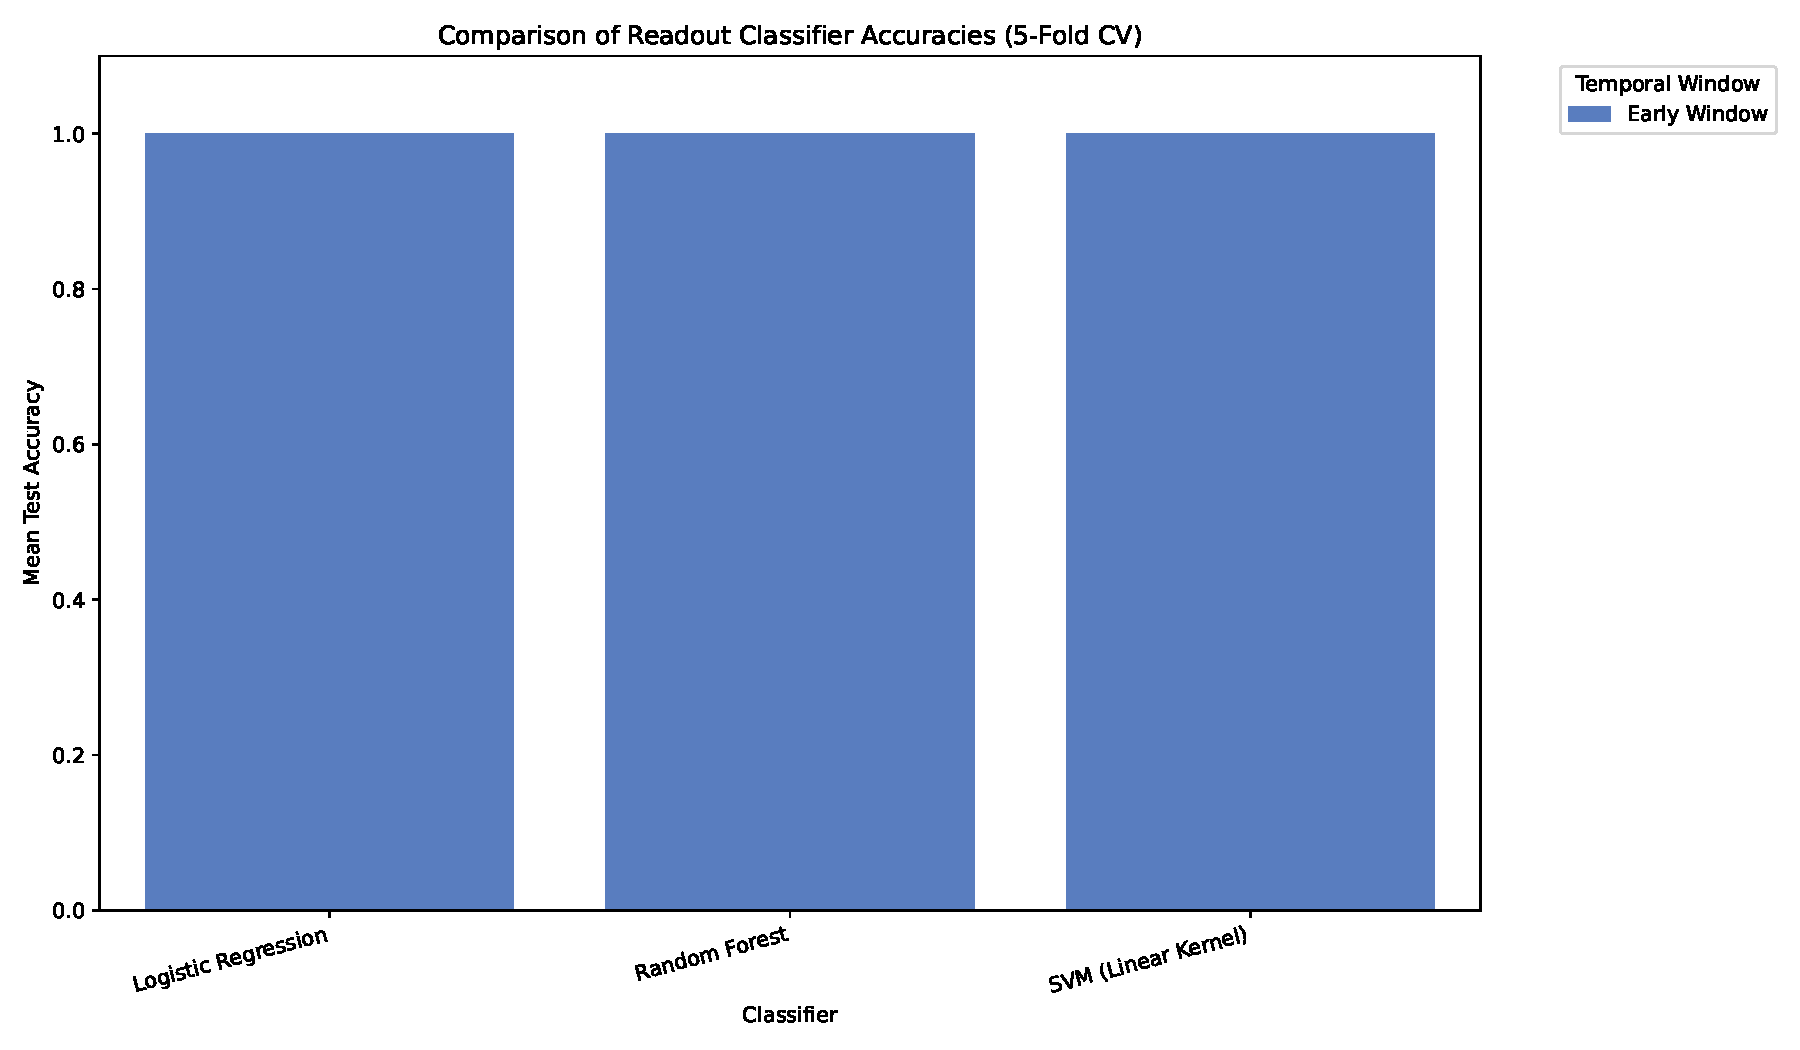
\includegraphics[width=0.8\textwidth]{pictures/chLSM/classifier_accuracy_comparison.pdf}
    \caption{Reported five-fold accuracy for three readouts on duplicated deterministic Early Window features. All classify the two unique feature vectors without error; the zero variance is not an independent generalization estimate.}
    \label{fig:m4_classifier_accuracy_comparison_actual}
\end{figure}

\begin{figure}[H]
    \centering
    \begin{subfigure}{0.48\textwidth}
        \centering
        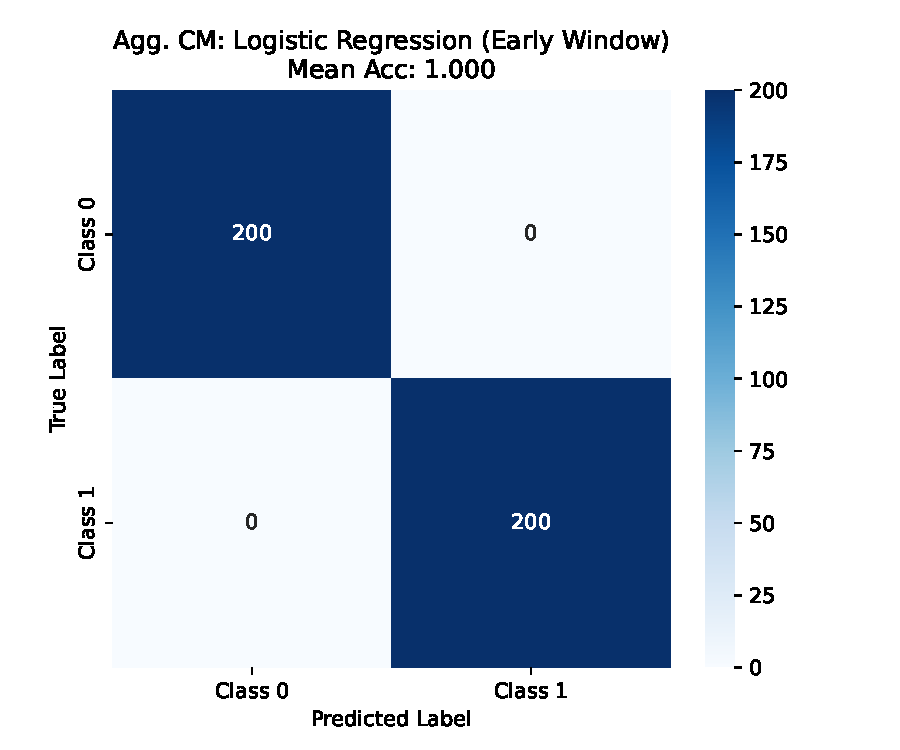
\includegraphics[width=\linewidth]{pictures/chLSM/cm_cv_logistic_regression_win_early_window.pdf}
        \caption{Logistic Regression (Acc: 1.000)}
        \label{fig:m4_cm_logreg_actual}
    \end{subfigure}
    \hfill
    \begin{subfigure}{0.48\textwidth}
        \centering
        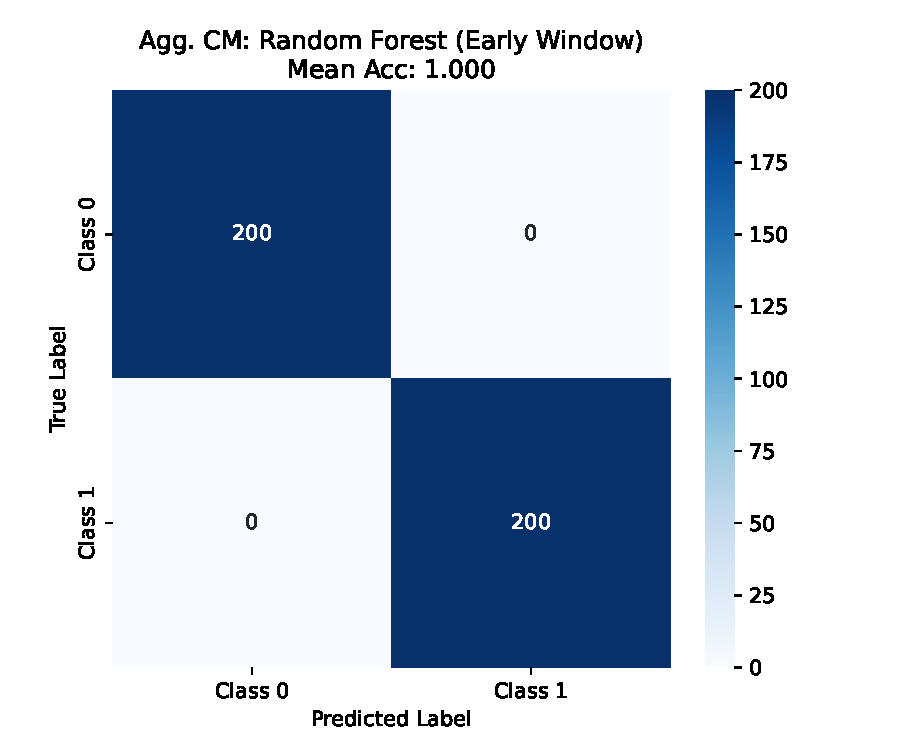
\includegraphics[width=\linewidth]{pictures/chLSM/cm_cv_random_forest_win_early_window.pdf}
        \caption{Random Forest (Acc: 1.000)}
        \label{fig:m4_cm_rf_actual}
    \end{subfigure}
    \vspace{1em}
    \begin{subfigure}{0.48\textwidth}
        \centering
        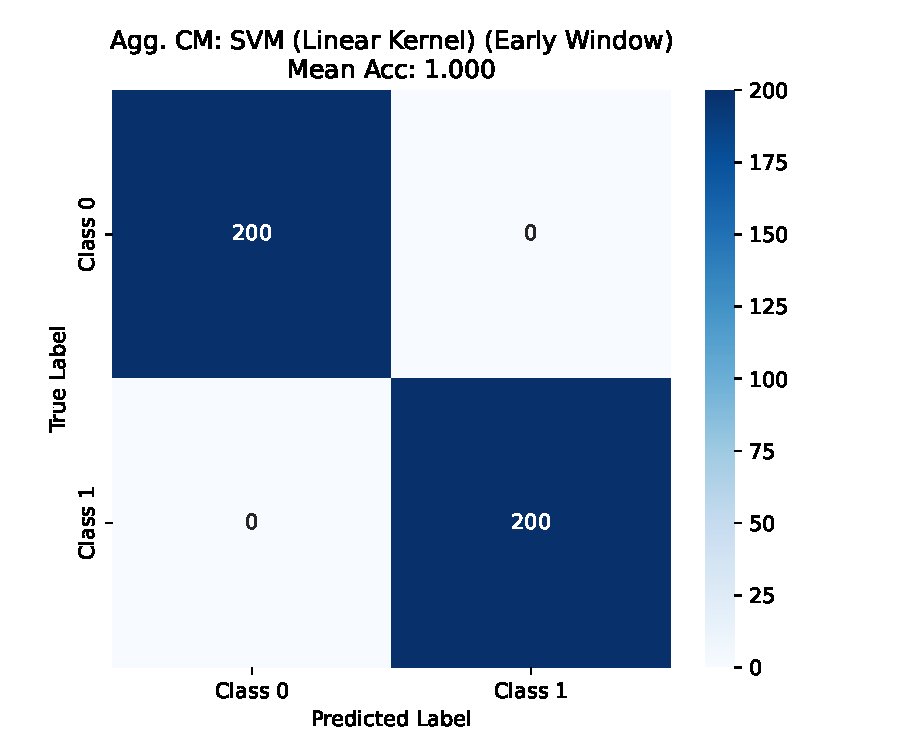
\includegraphics[width=\linewidth]{pictures/chLSM/cm_cv_svm_(linear_kernel)_win_early_window.pdf}
        \caption{SVM, Linear Kernel (Acc: 1.000)}
        \label{fig:m4_cm_svm_linear_actual}
    \end{subfigure}
    \caption{Aggregated five-fold confusion matrices. Counts reflect 200 duplicate copies of each of two unique feature vectors. $\beta=0.05$, $M_{\text{th}}=0.5$.}
    \label{fig:m4_confusion_matrices_all_actual}
\end{figure}

\subsection{Discussion and Significance}
\label{sec:module4_discussion}

\subsubsection{Observed Separability}

The two unique 512-dimensional feature vectors are separable by the fitted linear models, so Random Forest's nonlinear boundary was unnecessary for these stored points. Because the classes differ by a large scalar amplitude before entering the reservoir, the result is best treated as an implementation sanity check.

Mathematically, two finite sets are linearly separable if a hyperplane assigns every observed point to the correct side. The fitted linear models supply evidence of that property for the two stored vectors, but not for an unobserved distribution around them.

\subsubsection{Scope of the Controlled Result}

Three considerations define the scope of this result.

First, the task is a contrast between two constant-amplitude pulses with no additive noise or within-class variation. An energy detector on the raw input would also distinguish them perfectly. No raw-input linear baseline was fitted, so improvement in representation geometry is not established.

Second, a deterministic transformation cannot create label information absent from its input. The observed separability indicates that the selected readout can access the original amplitude contrast after reservoir processing; it does not quantify mutual information or improvement over raw input.

Third, separability of two deterministic pulse responses says little about noisy, heterogeneous EEG observations. The later SHAPE analyses therefore stand on their own and inherit the limitations documented in Chapter~\ref{chap:arspi_net}.

\subsubsection{What This Means for ARSPI-Net}

Within this scope, the result verifies that the implementation produces a nonconstant response that a simple readout can distinguish.

At the representation level, the selected operating point ($\beta=0.05$, $M_{\text{th}}=0.5$) maps the two amplitudes to distinct Early Window firing-rate vectors. Since the original one-dimensional amplitude contrast was already easy, the result does not show that the reservoir performed a harder representational task.

Architecturally, this is sufficient to pass a basic component test before forming channel-level features. It does not determine what a later graph model learns or show that graph propagation isolates inter-electrode relations.

The data-processing inequality remains a useful boundary: this fixed transformation cannot increase mutual information with the label. Any later change in Fisher ratio is a geometric statistic for a chosen representation, not evidence that information was created.


%% ===================================================================
%% CHAPTER SYNTHESIS
%% ===================================================================
\section{Chapter Synthesis: Toward ARSPI-Net Integration}
\label{sec:chapter3_synthesis}

The controlled observations inform, but do not validate, the later architecture. The membrane-decay sweep, threshold comparison, window comparison, and readout check each have an inspectable computational path. That traceability supports implementation auditing; it is not equivalent to a causal explanation of every population response, nor does it establish Koopman linearization, the Echo State Property, or clinical interpretability.

\subsection{Convergent Design Specifications}
\label{sec:design_specifications}

The experimental investigations across Modules~1--4 support the following provisional design conclusions:

\begin{enumerate}
    \item \textbf{Temporal control} (Module~1): $\beta=0.05$ gives intermediate persistence for the pulse and epoch tested here. It is carried forward as a provisional setting.

    \item \textbf{Response regime} (Module~2): $M_{\text{th}}=0.5$ produces amplitude-dependent spikes in the one tested realization. Stability relative to the high-threshold condition was not tested with matched seeds.

    \item \textbf{Window sensitivity} (Module~3): For the two deterministic responses, Early Window mean rates are separable and Late Window mean rates are not. Duplicate rows prevent a generalization claim.

    \item \textbf{Readout check} (Module~4): Linear readouts separate the two unique Early Window response vectors. The raw amplitude contrast is already separable, so no improvement over input space is established.
\end{enumerate}

\subsection{Operating Point Specification}
\label{sec:validated_configuration}

Table~\ref{tab:ch3_config} records the provisional configuration used to connect this characterization to Chapter~\ref{chap:embeddings}. That chapter separately evaluates 256 neurons, steps 10--70, and six-bin spike counts reduced to 64 dimensions.

\begin{table}[htbp]
\centering
\small
\caption{Provisional operating point from controlled characterization and later separately evaluated refinements.}
\label{tab:ch3_config}
\renewcommand{\arraystretch}{1.2}
\begin{tabularx}{\textwidth}{|>{\raggedright\arraybackslash}p{3.5cm}|>{\centering\arraybackslash}p{2.5cm}|>{\raggedright\arraybackslash}X|}
\hline
\textbf{Parameter} & \textbf{Value} & \textbf{Rationale} \\
\hline
Membrane decay ($\beta$) & 0.05 & Balances persistence and responsiveness; $\tau_m \approx 20$ steps (Module~1) \\
\hline
Firing threshold ($M_{\text{th}}$) & 0.5 & Produced graded spikes in one tested realization (Module~2) \\
\hline
Feature window & Steps 20--50 & Concentration of mean-rate discriminative content (Module~3) \\
\hline
Reservoir size & 512 neurons & Characterization configuration; 256 evaluated separately in Chapter~\ref{chap:embeddings} \\
\hline
Feature type & Mean firing rates & Baseline representation; refined to BSC$_6$ in Chapter~\ref{chap:embeddings} \\
\hline
Readout & Linear classifier & Separates the two unique controlled response vectors (Module~4) \\
\hline
\end{tabularx}
\end{table}

The readout result confirms only that the two stored response vectors are distinct in a linearly accessible way. The richer BSC$_6$ representation in Chapter~\ref{chap:embeddings} is motivated by the desire to preserve within-window timing, not by proof that this experiment improved the original geometry.

\subsection{Implications for the Dissertation}
\label{sec:ch3_implications}

The four modules provide component checks under controlled stimulation. Their implications are design hypotheses to be re-evaluated in later analyses.

\subsubsection{Architectural Implications}

Spike-based operation was retained because it supplies the event counts used by the downstream representation. The study did not establish a cross-seed robustness hierarchy, and the deterministic separability check does not determine what the later graph model learns.

\subsubsection{Methodological Implications}

The window comparison motivates testing temporally resolved counts rather than relying only on one mean rate. It does not show that later bins contain recoverable information; that would require a noisy, independently sampled task and a corresponding readout comparison.

No EEG window is inferred from the synthetic result alone. Chapter~\ref{chap:arspi_net} documents the window used for the available SHAPE summaries and treats the synthetic exercise as background rather than validation.

\subsubsection{Theoretical Implications}

Chapter~\ref{chap:dynamics} computes descriptive statistics of driven reservoir trajectories. Those statistics summarize the implemented transformation; they are not biomarkers, and this chapter does not prove the Echo State Property. The analysis window remains an explicit design choice whose consequences should be checked rather than inferred from thresholding alone.

Chapter~\ref{chap:synthesis} later compares dynamical and graph-derived summaries. The present chapter supplies implementation context for that comparison but does not establish that either summary has physiological meaning.

\subsection{Forward-Looking Design Principles}

The controlled characterization yields five limited design notes:
\begin{itemize}
    \item The selected low threshold produces the spike events required by the embedding pipeline; matched-seed robustness remains untested.
    \item Temporal windowing materially changes the chosen mean-rate readout and should be reported as part of the model specification.
    \item The two deterministic Early Window responses are linearly separable, but improvement over raw input is not established.
    \item Fixed weights and explicit update equations make the computational path inspectable. This is traceability, not a guarantee that each output has a unique physiological interpretation.
    \item The synthetic operating point is carried forward provisionally; the SHAPE results do not retroactively validate the simplified pulse experiments.
\end{itemize}

In summary, the chapter records how one fixed-weight reservoir implementation responds to controlled pulses and explains why $\beta=0.05$ and $M_{\text{th}}=0.5$ were carried forward. Unlike adaptive-reservoir approaches such as NeuCube \cite{kasabov_neucube_2014}, the realized weights here remain fixed after initialization. That choice makes the implemented transformation reproducible when the seed, weights, update rule, and preprocessing are retained, but it does not make the transformation completely interpretable or physiologically identified. Chapter~\ref{chap:embeddings} next evaluates compact temporal encodings for the downstream analyses.
